\documentclass{MScthesisITEM}

% this package is just to generate text for demo-purposes
\usepackage{blindtext}
\title{AUTONOMOUS LANDING OF UAV \\ PATH AND NAVIGATION} % The title of your assignement; NB use \newlinetitle to start a newline
\author{Kjetil Hope Sørbø} % Your firstname and lastname
\professor{Thor Inge Fossen, Tor Arne Johansen} % Affiliation = ITEM for instance
%\supervisor{Firstname Lastname, Affiliation}

%% Uncomment the following in case you want subfigures; note that there will be a warning for the caption package
 \let\subcaption\undefined
 \let\subfloat\undefined
 \usepackage[bf]{caption}
 \usepackage{subcaption}





\providecommand{\keywords}[1]{\textbf{\textit{Keywords:}} #1}

\DeclareGraphicsExtensions{.pdf,.jpg}
\graphicspath{{./figs/}}

\loadglsentries{glossary}
\makeglossaries


\begin{document}


\selectlanguage{english}
\pagenumbering{roman}
\pagestyle{plain}

%% Only for the project; comment out the line below for the master's thesis; the front page will be generated automatically by DAIM
\titleITEM

%% Only for the master's thesis; for the project report the description is taken from It's Learning and added by the department
% \selectlanguage{english} % Change to 'norsk' if you are writing in Norwegian
% \begin{titlingpage}

\noindent
\begin{tabular}{@{}p{4cm}l}
\textbf{Title:} 	& \thetitle \\
\textbf{Student:}	& \theauthor \\
\end{tabular}

\vspace{4ex}
\noindent\textbf{Problem description:}
\vspace{2ex}

\noindent \Blindtext[2][1]
\vspace{6ex}

\noindent
\begin{tabular}{@{}p{4cm}l}
\textbf{Responsible professor:} 	& \theprofessor \\
\textbf{Supervisor:}			& \thesupervisor \\
\end{tabular}

\end{titlingpage}
% \cleardoublepage

%% There must be an abstract in English, even though the main text is in Norwegian
\selectlanguage{english}
\pagestyle{empty}
\begin{abstract}
%Automatic landing of a fixed wing \acrfull{uav} in a net on a ship require an accurate positioning system. There exist today high-end systems with such capability for special applications, e.g military systems and costly commercial systems, which restrict the availability of such systems. To increase the general availability these systems must consist of low-cost components. Here, an alternative is the use of low-cost \gls{gnss} receivers and apply \gls{rtk-gps}, which can provide centimeter level position accuracy. However the processing time for the \gls{rtk-gps} system results in degraded accuracy when exposed to highly dynamical behaviour.
%
%This work present two alternative software and hardware position systems suitable for use in navigation system which apply \gls{rtk-gps}, namely \gls{rtklib} with a Ublox Lea M8T receiver and a Piksi system. Both the Piksi and the Ublox receiver are single-frequency \gls{gnss} receivers. These systems will in this work be compared and their individual capability to provide accurate position estimate will be evaluated. 
%
%The \gls{rtk-gps} system is implemented in DUNE (DUNE:Unified Navigation Environment) framework running on an embedded payload computer on-board an \gls{uav}.
%
%The performance of these position systems are in this work investigated by experimental testing. The testing showed that the \gls{rtklib} performed better than the Piski alternative, and further showed the tested navigation system provide sufficient quality for integration into a control and guidance system, allowing for automatic landing of an \gls{uav} in a net.

\end{abstract}
%\keywords{UAV,RTK-GPS,}

\cleardoublepage

%% Only for the master's thesis; if the main text is in English and you can write Norwegian, there must be an abstract in Norwegian as well.
% \selectlanguage{norsk}
% \pagestyle{empty}
\renewcommand{\abstractname}{Sammendrag}
\begin{abstract}
\noindent Denne avhandlingen presenterer ett bane- og navigasjonssystem, som brukes i et autonomt nett landingssystem for en fast-vinge \acrfull{uav}. Landingsbanen til en \gls{uav} kan konstrueres som en rett linjet bane, men for at en \gls{uav} skal kunne følge landingsbanen må \gls{uav}en være i en posisjon hvor det finnes en mulig bane til landingsbanens start posisjon. Dette motiverer utviklingen av en innflyvingsbane logikk mot landingsbanen sin inngangs posisjon fra hvilken som helst innledende startposisjon i luftrommet.

I tillegg til et bane genererende system trenger \gls{uav}en ett robust høy nøyaktighets navigasjonssystem. Dette gjøres med å bruke \acrfull{rtk-gnss}, som kan gi centimeter nøyaktighet. En ulempe med \gls{rtk-gnss} er at det kan miste lås på satellitter som fører til tap av funksjonalitet. I dette arbeidet kompenseres dette ved å benytte et sekundært \acrfull{gnss} system. For å håndtere tap av \gls{rtk-gnss} er et robust \gls{rtk-gnss} system foreslått, hvor tidligere gyldige \gls{rtk-gnss} posisjon løsninger er kombinert med det sekundære \gls{gnss} systemet, for å bli brukt til å kompensere det eksterne navigasjon systemet. Denne kompensatoren er utformet slik at det eksterne navigasjonssystemet får samme nøyaktighets nivå som \gls{rtk-gnss} i en kort periode, inntil enten \gls{rtk-gnss} kommer tilbake eller blir frakoblet. Med denne kompensatoren blir navigasjonssystemet til \gls{uav}en robust mot korte tap av \gls{rtk-gnss}, og tilgjengeligheten til \gls{rtk-gnss} er utvidet.

Både eksperimentell testing og \acrfull{sil} verifikasjon har blitt utført for å teste \gls{uav}ens evne til å lande i et stasjonært nett plassert på en tilfeldig posisjon. For å bedre navigasjon og ytelse, har en mobil sensor enhet blitt benyttet for å få posisjonen til nettet. Denne sensoren enheten ble benyttet under testing, hvor den viste seg å gi det tiltenkte bidraget.
\end{abstract}
% \cleardoublepage

\selectlanguage{english}% Change to 'norsk' if you are writing in Norwegian

%\renewcommand{\abstractname}{Preface}
\begin{abstract}
\noindent This thesis is submitted in partial fulfillment of the requirements for the Master of Science degree at the Norwegian University of Science and Technology.

The work presented in this thesis has been carried out at the Department of Engineering Cybernetics, and would not have been possible without the inputs and contributions from many of its associates. First, I would like to thank Professor Tor Arne Johansen and Professor Thor Inge Fossen for their inspiring ideas and guidance into the academic world. A huge thanks goes to Kristian Klausen for his invaluable help and guidance at the UAV-Lab. Furthermore I want to thank the UAV-pilots Lars Semb and Pål Kvaløy for excellent flying. I would also like to thank my fellow MSc. students at the UAV-Lab. They gave me invaluable feedback and made a coordinated development of the autonomous landing system possible.

Finally I want to thank my parents and brothers for their never-ending support and guidance.
\begin{center}
\emph{Trondheim, June, 2016} \\
\emph{Kjetil Hope Sørbø}
\end{center}
\end{abstract}
%\cleardoublepage

% similarly you may add a separate acknowledgments page

\tableofcontents*
\cleardoublepage

%% include if relevant
%\listoffigures
%\cleardoublepage
%
%%% include if relevant
%\listoftables
%\cleardoublepage

%% include if relevant
%\listofalgorithms
%\addcontentsline{toc}{chapter}{List of Algorithms}
%\cleardoublepage

%% include if relevant
%\printglossary[title=List of Symbols, style=long]
%\cleardoublepage
\glsaddall[]

%% include if relevant
\printglossary[title=Acronyms,type=\acronymtype] % prints just the list of acronyms


\cleardoublepage



\pagenumbering{arabic}
\pagestyle{ruled}
%===================================== CHAP 1 =================================
\chapter{Introduction}
\section{Background}
Recent development of flying \glspl{uav} has been recognized to provide an attractive alternative to work previously performed by manned operations. Typical work which has attracted attention includes inspection, aerial photography, environmental surveillance and search and rescue. Today \gls{uav} operation are becoming more autonomous, however in order to become fully autonomous a fixed wing \gls{uav} must be able to perform a autonomous landing.

An important premise for successful and safe \gls{uav} operation, is the provision of a robust system for safe landing of the \gls{uav} following completed operations. A autonomous landing system require a path generation system that can create a flyable landing path during flight operation from any initial position. In addition the navigation system must have centimeter level accuracy in order for the \gls{uav} to perform a autonomous landing in a net. However with a accurate navigation system the case of what to do when the positioning system degenerates must be resolved such that system failure does not occur. An other premise is that the position of the net is known, and available for the path system. With a known position of the landing net the \gls{uav} must gracefully perform a graceful decent, preferable a glide slope towards the landing net position. The length of the glide slope will be limited by the operator, which dictates that the \gls{uav} must be in the correct pose before starting the decent.
\section{Literature review}
There has been perform several studies on autonomous landing system, and there currently exist commercial available system. However these are typical expensive, and mostly focused on either military or air traffic industry. An available system for \glspl{uav} is the SkyHook that apply INS/\gls{gps}\citep{SkyHook}, however this system require expensive equipment and is limited to a few \gls{uav} systems. The limitation on type of \gls{uav} and high cost restricts the usage of the recovery system, and motivates the research of a low cost recovery system for fixed wing \gls{uav}.

Studies that has been performed on autonomous landing has mostly focused on vision-based guidance, due to previously limited accuracy in low-cost \gls{gnss} receiver system, which is typically single frequency receivers. In the paper \citep{barber2007autonomous} a landing system was proposed that compared the use of barometric pressure measurement and optic-flow measurement for estimation of height above ground. The landing path composed of a spiral path down to a given altitude where a glide slope was used to guide the MAV down to the landing area. The papers showed that optic-flow measurement reduced the average landing error with several meters, however the technique used to guided the \gls{uav} is not suitable for precision landing due to large average error from target. A low cost recovery system for fixed wing \gls{uav} is proposed in the paper \citep{kim2013fully}, where computer vision is used to find and identify the recovery net. The system was successful in performing a autonomous landing, however it require that the visual image is sent from the \gls{uav} to a ground station. In addition the system require a clear image in order to calculate guidance command for the \gls{uav}, which restricts when the system can used. In the paper \citep{huh2010vision} a vision-based landing system is presented which was successful in performing a automatic landing. The system was aided by a standard IMU and GPS, together with a vision system relaying on color and moments based detection. The system is sensible to lighting condition, however a filtering rule was used to find the landing area. The sensibility to lighting condition is a disadvantage with vision-based guidance system, and therefore it's preferable to create a high accurate positioning system.

A net recovery system for \gls{uav} with single-frequency \gls{rtk-gps} was described in the paper \citep{skulstad2015net}, which was a result of the work done in the master thesis \citep{Skulstad&Syversen}. The system presented applied RTKLIB together with low-cost single frequency \gls{gps} receivers as navigation system with a customized Ardupilot software. The complete system was able to perform a net landing, however the result showed that further work would require better controllers, and a more robust navigation system. A continuation of the work done in \citep{Skulstad&Syversen} was done in \citep{Froelich}. The work simulated a autonomous net landing, however no physical experiment was perform. The result in the work indicated that further work on the controllers was required, in addition to the landing path which was not suited for a Visual Line Of Sight  (VLOS) \gls{uav} operation due to no spacial restrictions.
\section{Contributions}
The objective of this work is to design, implement and test a autonomous landing system for fixed wing \gls{uav}. The focus area for this work has been the design and implementation of a landing plan, and a high accurate navigation system. The landing path generator is a improved version of the landing path used in \citep{Skulstad&Syversen} moved into the DUNE environment, and combined with the landing path generator interface created in the master thesis \citep{Froelich}. The navigation system continues the work started in the master thesis \citep{Spockeli}, where \gls{rtk-gnss} was made available to the DUNE environment. The guidance and control system used during the testing of the system was developed at the UAVLab by a fellow master student. The contributions of this thesis are a landing plan generator, a navigation system able to provide high accurate position and velocity information, a redundancy strategy for short loss of \gls{rtk-gnss}, a mobile sensor unit used as a \gls{gps} reference location for net placement and a experimental testing and operational study of the autonomous landing system, summarised as follows:
\begin{enumerate}
\item \textbf{A landing plan generator} has been created, which guaranty a flyable path from any initial position to a landing zone, with a specified decent angle. The landing plan generator has been implemented in the DUNE runtime environment, which is capable to be used in both a stationary and moving net landing. In addition to the implementation of the landing plan a \textbf{\gls{api}} has been created to generate a landing plan.
\item \textbf{A navigation state control system} has been created to manage which positioning system should be used in the DUNE environment. The state machine is designed to switch between the position and velocity information provided by the external navigation system and the \gls{rtk-gnss} position and velocity solution.
\item \textbf{Increased the robustness of the \gls{rtk-gps}} by creating a bias estimator, which estimate the bias between \gls{rtk-gps} and a standalone \gls{gps}. The bias is used to compensate the external navigation position solution such that the external navigation position solution equals a FIX \gls{rtk-gnss} position solution.
\item \textbf{A navigation state monitor interface} has been created to provide a visual indicator of which navigation system that is used in the DUNE environment. The monitor is color coded such that changes in the state of the navigation system detected with more ease.
\item \textbf{A mobile sensor with \gls{rtk-gps}} has been created to be a reference position for a stationary net. The mobile sensor unit can be place on a runway, and used as a reference point for net placement in the command and control monitor, and provide accurate position solution for placement of net through the use of \gls{rtk-gnss}.
\item \textbf{Experimental testing} of the navigation system and landing path generator in the field. The autonomous landing system was tested on the Agdenes airfield with a virtual net placed $25 m$ above the runway. Test result gathered from the field test has been used in a \textbf{operational study} on performance and  feasibility of a autonomous landing at Agdenes airfield.
%\item Finally statistical data on the performance of the X8 during landing during landing has been gather to be used in further work in further developing the landing system.
\end{enumerate}
\section{Outline}
Chapter 2 outlines two path planing strategies which is used in the development of the landing path system. The chapter also contains a model of a \gls{mav}.

Chapter 3 proposes a path and navigation system for a autonomous landing system. The landing path system is separated into two planes, which is the lateral and longitudinal plane. The lateral path is created as a Dubins path, and the longitudinal path is created as a straight line path. The navigation system is controlled by a state machine which controls the source of the positioning and velocity solution, in addition to increasing the robustness of the \gls{rtk-gnss}.

Chapter 4 outlines the software used to create and test the autonomous landing system as well as the hardware configuration used as a basis for the X8 fixed wing \gls{uav}.

Chapter 5 outlines the implementation details of the path and navigation system, including simulation verification of the system.

Chapter 6 present experimental testing of the path and navigation system in the field 

Chapter 7 present the closing discussion with conclusion and recommendation for further work.
\cleardoublepage
\chapter{Basis and modelling}
\section{UAV model}
A fixed wing \gls{uav} model is presented in \citep{beard2012small}, where the kinetic equations of a general \gls{mav} is proposed. The kinetic equations used to described a general \gls{mav} can represent a fixed wing \gls{uav} given that the size of the \gls{uav} is small enough, which is the case with the \gls{uav} used in this thesis. The kinematic equations used to describe a \gls{mav} is given as:
\begin{subequations}
\label{eq:kinematics}
\begin{align}\label{eq:kinematicsPosition}
& \begin{bmatrix}
\dot{x} \\
\dot{y} \\
\dot{z}
\end{bmatrix}
=
 \mathbf{R}(\mathbf{\Theta})_{Body}^{NED}\begin{bmatrix}
 u \\
 v \\
 w
 \end{bmatrix} \\
& \begin{bmatrix}
\dot{\phi} \\
\dot{\theta} \\
\dot{\psi}
\end{bmatrix}
= 
\mathbf{T}(\mathbf{\Theta}_{nb})\begin{bmatrix}
p \\
q \\
r
\end{bmatrix}\label{eq:kinematicsAttitude}
\end{align}
\end{subequations}
where $\mathbf{R}(\mathbf{\Theta})_{Body}^{NED}$ is the rotation matrix from the body frame to the \gls{ned} frame, with $\mathbf{\Theta} = \begin{bmatrix}
\phi & \theta & \psi
\end{bmatrix}^T.$ The transformation matrix $\mathbf{T}(\mathbf{\Theta}_{nb})$ is given in \citep{fossen2011handbook} as:
\begin{equation}
\mathbf{T}(\mathbf{\Theta}_{nb}) = \begin{bmatrix}
1 & \sin(\phi)\tan(\theta) & \cos(\phi)\tan(\theta) \\
0 & \cos(\phi) & -\sin(\phi) \\
0 & \frac{\sin(\phi)}{\cos(\theta)} & \frac{\cos(\phi)}{\cos(\theta)}
\end{bmatrix}
\end{equation}
The kinetic equations presented from \citep{beard2012small} are given in the body frame, a frame fixed to the body of the vehicle and rotated relative to an inertia frame, e.q the Earth center. The kinetic equations are given as:
\begin{subequations}
\label{eq:kinetics}
\begin{align}
\begin{bmatrix}
F_x \\
F_y \\
F_z
\end{bmatrix}
&= \mathbf{R}(\mathbf{\Theta})^{Body}_{NED}\begin{bmatrix}
0 \\
0 \\
mg
\end{bmatrix} - \frac{1}{2} \rho V_a^2 S \mathbf{R}(\alpha)_{Stability}^{Body}\begin{bmatrix}
F_{Drag} \\
0 \\
F_{Lift}
\end{bmatrix}\\ &+ \frac{1}{2} \rho V_a^2 S \begin{bmatrix}
0 \\
C_y(\beta,p,r,\delta_a,\delta_r) \notag\\
0
\end{bmatrix} + \frac{1}{2} \rho S_{Prop} C_{Prop} \begin{bmatrix}
(K_{Motor}\delta_t)^2-V_a^2 \\
0 \\
0
\end{bmatrix}\\
\begin{bmatrix}
 L \\
 M \\
 N 
 \end{bmatrix} &= \frac{1}{2} \rho V_a^2S\begin{bmatrix}
 C_L(\beta,p,r,\delta_a,\delta_r) \\
 C_M(\alpha,q,\delta_e) \\
 C_N(\beta,p,r,\delta_a,\delta_r)
 \end{bmatrix} + \begin{bmatrix}
 -k_{T_p}(K_\Omega\delta_t)^2 \\
 0 \\
 0
 \end{bmatrix}
\end{align}
\end{subequations}
where $\rho$ is the air density in $kg/m^3$,$mg$ is the weight of the \gls{mav}, $S$ is the platform area of the \gls{mav} wing, $C_i$ are nondimensional aerodynamic coefficients and $V_a$ is the speed of the \gls{mav} through the surrounding air. $\alpha$ and $\beta$ is the attack and side slip angle respectively. $F_{Drag}$ is the drag force acting on the fuselage, and $F_{Lift}$ is the lift force. $\mathbf{R}(\alpha)_{Stability}^{Body}$ is the rotation matrix from the stability frame to the body frame. The stability frame is orientated with respect to the \gls{mav} movement through the surrounding air, defined as a standard rotation around the y-axis of the body frame. $S_{Prop}$ is the area swept out by the propeller, and $K_{Motor}$,$K_{T_p}$ and $K_\Omega$ are propeller specific constants. The control surface on the \gls{mav} is defined into two groups; the wings and the rudder. On the rudder $\delta_e$ controls the elevator deflection and $\delta_r$ the rudder deflection. For the wings $\delta_a$ is the control input from the aileron deflection, while $\delta_t$ is the throttle control input.
\section{Landing path modelling}
A landing path can be viewed as a path following problem where the \gls{uav} attempts to follow a desired path without a time demand. A minimum requirement for a path is that the path segments are connected, where the connection level can be described by the path smoothness. Smoothness can be described with parametric continuity, denoted $C^n$ were n is the degree of smoothness. The order of n implies that the n first parametric derivatives match at a common point for two subsequent paths \citep{barsky1989geometric}. Geometric continuity is a relaxed form of parametric continuity in which discontinuity in speed is allowed. Table \ref{TB:SmoothnessDescriptions} of geometric and parametric continuity, lists the requirement for each smoothness level, which is based on definitions presented in \citep{barsky1989geometric}. Geometric continuity is sufficient for a path following system. Geometric continuity is denoted as $G^n$ were n is the order of continuity.
\begin{table}[H]
\begin{center}
\begin{tabular}{| l | l |}
\hline
\textbf{Geometrical smoothness level} & \textbf{Description} \\ \hline
$G^0$ & All subpaths are connected \\ \hline
$G^1$ & The path-tangential angle is continuous \\ \hline
$G^2$ & The center of curvature is continuous \\ \hline
\textbf{Parametric smoothness level} & \textbf{Description} \\ \hline
$C^0$ & All subpaths are connected \\ \hline
$C^1$ & The velocity is continuous \\ \hline
$C^2$ & The acceleration is continuous \\ \hline
\end{tabular}
\end{center}
\caption{Smoothness definitions for both parametric and geometric}
\label{TB:SmoothnessDescriptions}
\end{table} 
The definition used for path in this thesis is equation 1.2 in \citep{tsourdos2010cooperative} which state:
\begin{equation}
P_s(x_s,y_s,z_s,\theta_s,\psi_s) \xrightarrow{r(\varpi)} P_f(x_f,y_f,z_f,\theta_f,\psi_f)
\end{equation}
where the subscripts $s$ and $f$ denotes the start pose and finish pose respectively with $r(\varpi)$ as the path and $\varpi$ the path variable.

\subsection{Straight lines}
The simplest path from $P_s$ and $P_f$ is a straight line path between the poses. A straight line path is given. For simplicity and without loss of generality the path is reduced to a 2 dimensional case: 
\begin{subequations}
\begin{align}
& x(\varpi) = a_x\varpi + b_x \\
& y(\varpi) = a_y\varpi + b_y 
\end{align}
\end{subequations}
with $ \varpi \in [0,1] $, where $\varpi$ has not necessary a physical meaning. Then the parametrisation of the straight line becomes:
\begin{subequations}
\begin{align}
P(0) &= \begin{bmatrix}
x(0) \\
y(0)
\end{bmatrix} = \begin{bmatrix}
b_x \\
b_y
\end{bmatrix} = \begin{bmatrix}
x_s \\
y_s
\end{bmatrix} \\
P(1) &= \begin{bmatrix}
x(1) \\
y(1)
\end{bmatrix} = \begin{bmatrix}
a_x + b_x \\
a_y + b_y
\end{bmatrix} = \begin{bmatrix}
x_f \\
y_f
\end{bmatrix} \rightarrow \begin{bmatrix}
a_x \\
a_y
\end{bmatrix} = \begin{bmatrix}
x_f - b_x \\
y_f - b_y
\end{bmatrix}
\end{align}
\end{subequations}
Further the path tangential for a straight line path is given as:
\begin{equation}
\psi(\varpi) = \atan2(a_y,a_x)
\end{equation}
which shows that the path-tangential for a straight line path is discontinues as seen in figure \ref{Fig:Path-tangential}. This defines a straight line path with the smoothness of $G^0$, allowing the path to be used in a path following system, however with discontinuity in the path-tangential. A straight line path is shown in  figure \ref{Fig:StraightLinePath}.
%\begin{figure}[H]
%\centering
%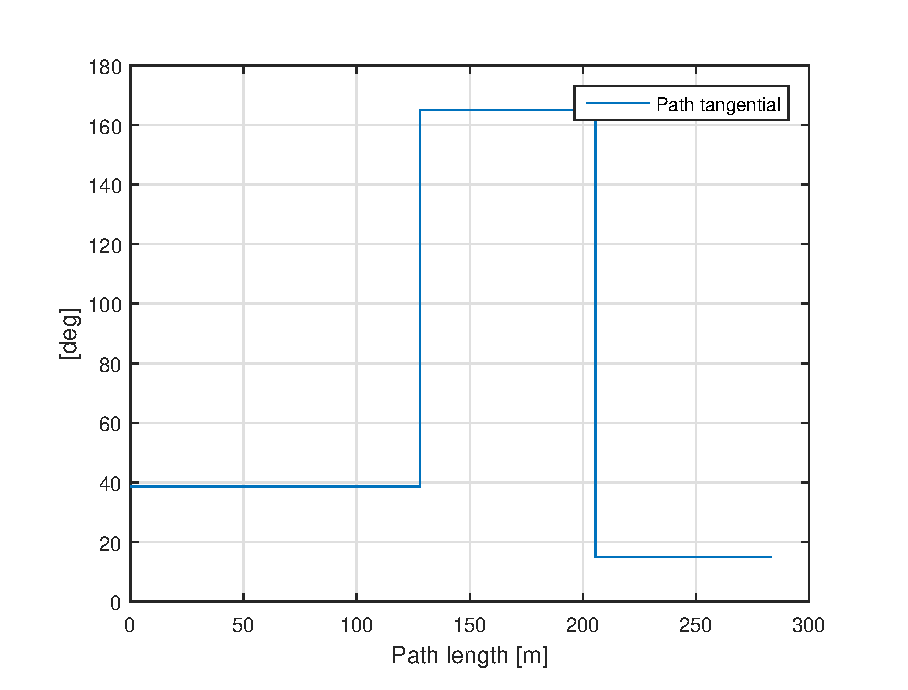
\includegraphics[scale=0.5]{figs/TheoryPlot/TangentialStraight.eps}
%\caption{Path-tangential to a straight line path}
%\label{Fig:Path-tangential}
%\end{figure}
%\begin{figure}[H]
%\centering
%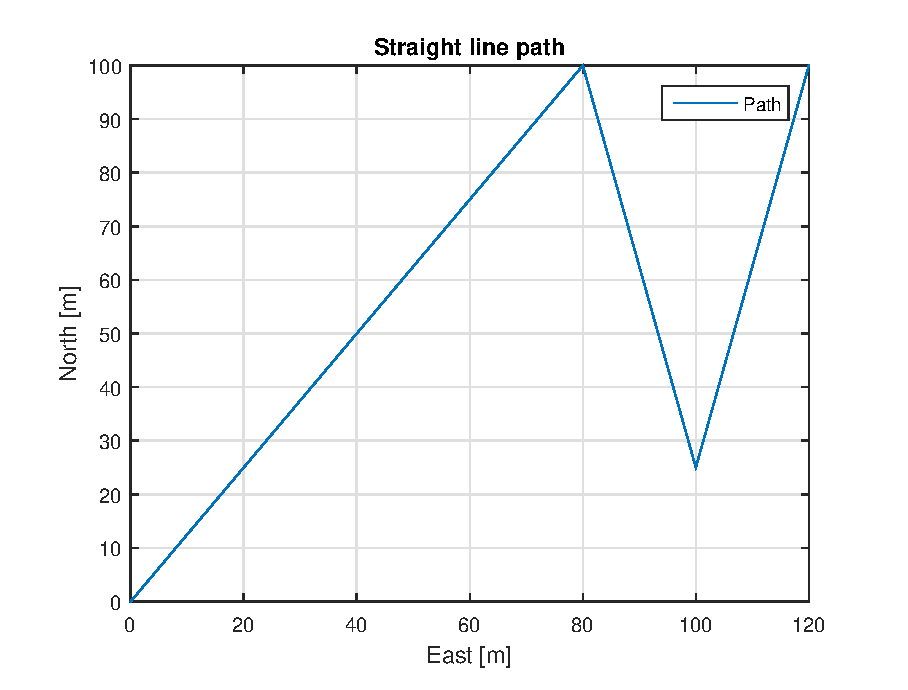
\includegraphics[width=0.5\textwidth]{figs/TheoryPlot/StraightLine.eps}
%\caption{Straight line path}
%\label{Fig:StraightLinePath}
%\end{figure}

\begin{figure}[H]
\centering
\begin{subfigure}{0.49\textwidth}
		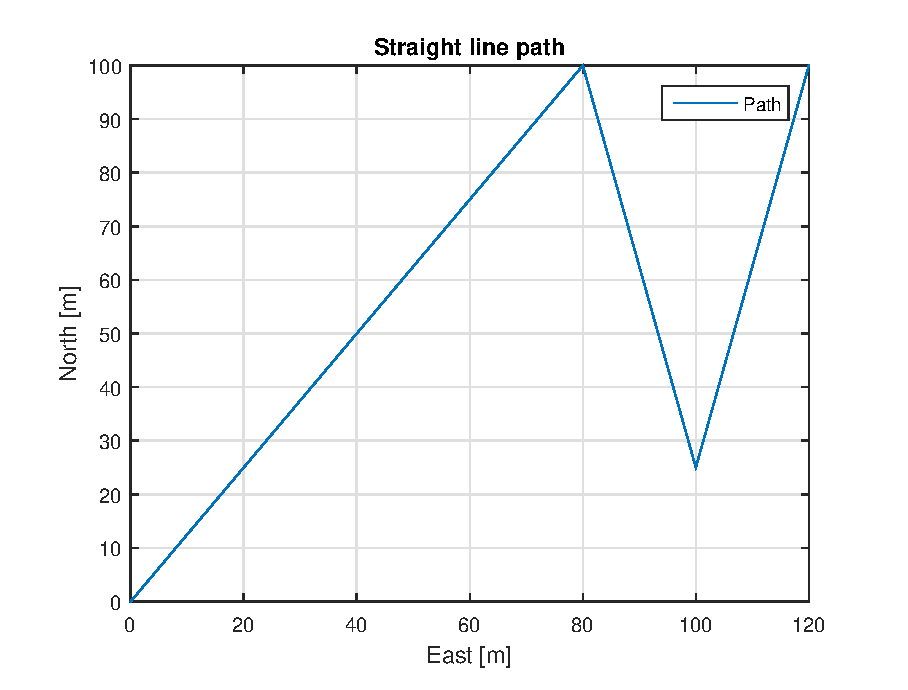
\includegraphics[width=\textwidth]{figs/TheoryPlot/StraightLine.eps}
\caption{Straight line path}
\label{Fig:StraightLinePath}
\end{subfigure}
\begin{subfigure}{0.49\textwidth}
		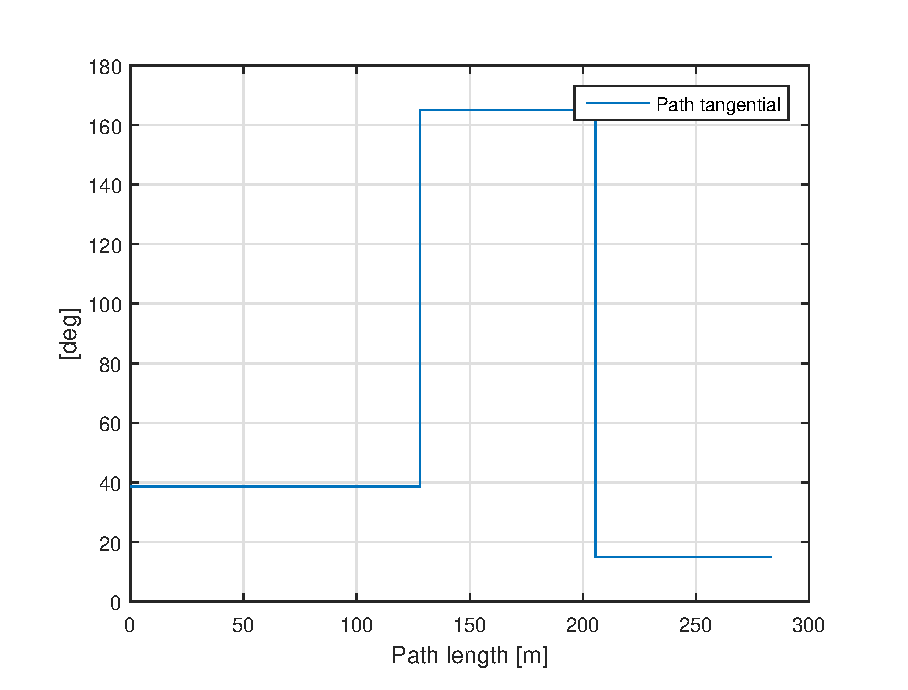
\includegraphics[width=\textwidth]{figs/TheoryPlot/TangentialStraight.eps}
		\caption{Path-tangential to a straight line path}
		\label{Fig:Path-tangential}
\end{subfigure}
\caption{Straight line path with path tangential}
\label{Fig:StraightLine}
\end{figure}

\subsection{Dubins path}\label{S:DubinsPath}
An alternative to a straight line path is a path constructed by straight lines and circle, like the Dubins path proposed in the paper \citep{dubins1957curves}. This paper showed that the shortest possible path for a particle that moved with unit speed with maximum curvature would consist of two circles and a straight line which is tangential to both circles.

A Dubins path constructed with the final orientation fixed has four ways to be constructed, determined by the rotation directions. The four rotation combination with fixed finish orientation are given in table \ref{Tb:DubinsTurningDirection}.
\begin{table}[H]
\centering
\begin{adjustbox}{max width=\textwidth}
\begin{tabular}{ | l |}
\hline
Right to Right \\
Right to left \\
Left to Right \\
Left to left \\ \hline
\end{tabular}
\end{adjustbox}
\caption{Turning direction for Dubins path with fixed final orientation}
\label{Tb:DubinsTurningDirection}
\end{table}
The equations used to construct a Dubins path are found in \citep{tsourdos2010cooperative} section 2.2.1, with a constructed path shown in figure \ref{Fig:DubinsPath}. In figure \ref{Fig:DubinsPath} the whole line is the path, where the doted lines used express the parameter used to construct the path.
\begin{figure}[H]
\def\svgwidth{\textwidth} % Defining the width since Inkscape hasn't done this yet in the .pdf_tex file
\input{InkFig/DubinsPath.pdf_tex}
\caption{The whole line is the Dubins path, while the doted lines are used to express the parameters used to construct the path}
\label{Fig:DubinsPath}
\end{figure}
Dubins path is constructed by first determine the start and finish turning circle center. The centres are found with the equations:
\begin{subequations}
\begin{align}
X_{cs} &= X_s - R_s\cos(\psi_s \pm \frac{\pi}{2}) \\
Y_{cs} &= Y_s - R_s\sin(\psi_s \pm \frac{\pi}{2}) \\
X_{cf} &= X_f - R_f\cos(\psi_f \pm \frac{\pi}{2}) \\
Y_{cf} &= Y_f - R_f\sin(\psi_f \pm \frac{\pi}{2})
\end{align}
\end{subequations}
where $R_s$ and $R_f$ are the radius of the start and final turning circle respectively, with $\psi_s$ and $\psi_f$ as the start and finish orientation. The centres for the start and finish turning circles are defined as:

\begin{align}
& \mathbf{O}_{cs} =
\begin{bmatrix}
X_{cs} \\
Y_{cs}
\end{bmatrix} \\
& \mathbf{O}_{cf} =
\begin{bmatrix}
X_{cf} \\
Y_{cf}
\end{bmatrix}
\end{align}
Continuing the centres $O_{cs}$ and $O_{cf}$ are connected with a centreline $c$, where the length is given as:
\begin{equation}
|c| = ||\mathbf{O}_{cs} - \mathbf{O}_{cf}||_2
\end{equation}
where $||\cdot||_2$ is the second norm. Continuing the arc exit and entry point for the start and finish circles are calculated by first applying the equations:
\begin{subequations}
\begin{align}
& \alpha = \arcsin\left(\frac{R_f-R_s}{|c|}\right) \\
& \beta = \arctan\left(\frac{Y_{cf}-Y_{cs}}{X_{cf}-X_{cs}}\right)
\end{align}
\end{subequations}
where $\alpha$ is the angle between the length of the center line between the two circles, and the length of the line from the start circle to the exit tangent point. $\beta$ is the angle of the center line with respect to the inertial frame. The exit and entry tangent point is found with the use of table \ref{Tb:ExitEntryTangent}.
\begin{table}[H]
\begin{center}
\begin{tabular}{ | l | l |}
\hline
& \textbf{Turn angle} \\ \hline
$\phi_{right}$ & $\alpha + \beta + \frac{\pi}{2}$ \\
$\phi_{left}$ & $\beta - \alpha + \frac{3\pi}{2}$ \\ \hline
\end{tabular}
\caption{Turn angle}
\label{Tb:ExitEntryTangent}
\end{center}

\end{table}
With the angle of the exit and entry tangent point the points are given as:
\begin{subequations}
\begin{align}
& x_{P_\chi} = x_{cs} + R_s\cos(\phi) \\
& y_{P_\chi} = x_{cs} + R_s\sin(\phi) \\
& x_{P_N} = x_{cf} + R_f\cos(\phi) \\
& y_{P_N} = x_{cf} + R_f\sin(\phi)
\end{align}
\end{subequations}
which is used to define the exit and entry points as:
\begin{subequations}
\begin{align}
\mathbf{P}_{\chi} &= \begin{bmatrix}
x_{P_\chi} \\
y_{P_\chi}
\end{bmatrix} \\
\mathbf{P}_N &= \begin{bmatrix}
x_{P_N} \\
y_{P_N}
\end{bmatrix}
\end{align}
\end{subequations}
The length of the Dubins path is the sum of the length of the two circle arcs and the straight line, given as:
\begin{equation}
d = R_s\phi_s + d_t + R_f\phi_f
\end{equation}
where $d_t = ||\mathbf{P}_N-\mathbf{P}_{\chi}||_2$, $\phi_s$ and $\phi_f$ is the arc angle for the start and finish circle respectively. The path-tangential of the Dubins path is given as:
\begin{equation}
\psi = \atan2(1,-tan(\phi))
\end{equation}
which determine that the path-tangential is continues, i.e. Dubins path $G^1$. The path-tangential for Dubins path is shown in figure \ref{Fig:Path-tangentialDubin}.
\begin{figure}[H]
\centering
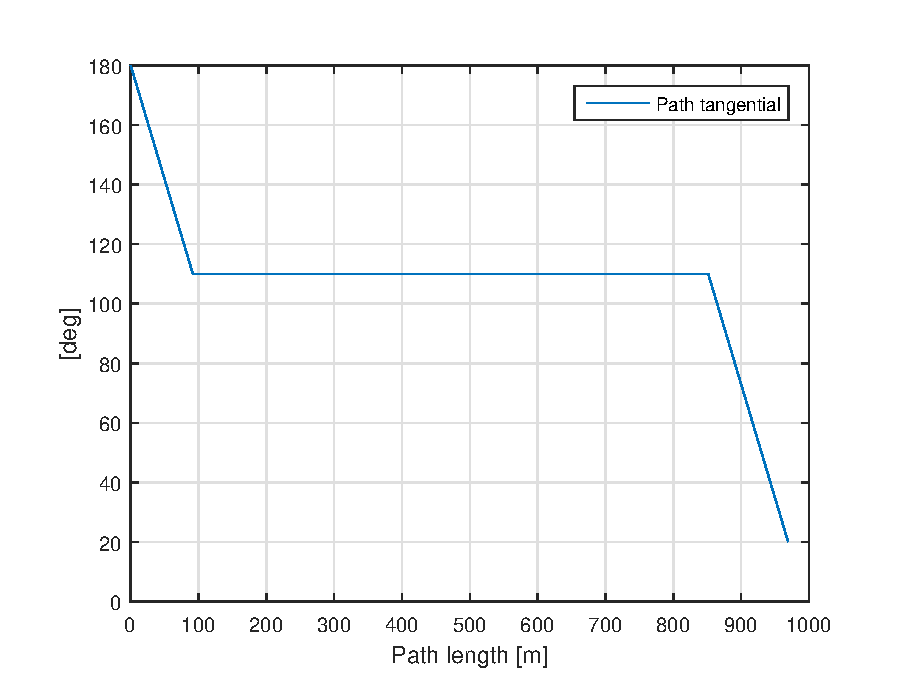
\includegraphics[scale=0.7]{figs/TheoryPlot/tangentialDubin.eps}
\caption{Path-tangential for a Dubins path}
\label{Fig:Path-tangentialDubin}
\end{figure}
\cleardoublepage
%\chapter{Path planning theory}
An autonomous system must be able to create a plan on how the system should move around in the surrounding environment in a feasible way. A minimum requirement for a path is that it is connected. The connection level can be described by the paths smoothness.
Parametric continuity is denoted $C^n$ were n is the degree of smoothness. The order of n implies that the n first parametric derivatives match at a common point for two subsequent paths \citep{barsky1989geometric}. Geometric continuity is a relaxed from of parametric continuity in witch discontinuousness in speed is allowed. A table of geometric and parametric continuity lists the requirement for each smoothness level \ref{TB:SmoothnessDescriptions}, which is based definitions presented in \citep{barsky1989geometric}.
Geometric continuity is sufficient for a path following system, witch is the main focus of this thesis. Geometric continuity is denoted as $G^n$ were n is the order of continuity.

\begin{table}[H]
\begin{center}
\begin{tabular}{| l | | l |}
\hline
\textbf{Geometrical smoothness level} & \textbf{Description} \\ \hline
$G^0$ & All subpaths are connected \\ \hline
$G^1$ & The path-tangential angle is continuous \\ \hline
$G^2$ & The center of curvature is continuous \\ \hline
\textbf{Parametric smoothness level} & \textbf{Description} \\ \hline
$C^0$ & All subpaths are connected \\ \hline
$C^1$ & The velocity is continuous \\ \hline
$C^2$ & The acceleration is continuous \\ \hline
\end{tabular}
\end{center}
\caption{Smoothness definitions}
\label{TB:SmoothnessDescriptions}
\end{table} 

The definition used for path in this thesis is equation 1.2 in \citep{tsourdos2010cooperative} which state:
\begin{equation}
P_s(x_s,y_s,z_s,\theta_s,\psi_s) \xrightarrow{r(q)} P_f(x_f,y_f,z_f,\theta_f,\psi_f)
\end{equation}
where the subscripts $s$ and $f$ denotes the start pose and finish pose respectfully with $r(q)$ as the path.

\section{Straight lines}
The simplest form on path is a straight line between $P_s$ and $p_f$. The straight line is given as 
\begin{subequations}
\begin{align}
& x(s) = a_xs + b_x \\
& y(s) = a_ys + b_y 
\end{align}
\end{subequations}
with $ s \in [0,1] $, where $s$ has not necessary a physical meaning. Then the parametrisation of the straight line is:
\begin{subequations}
\begin{align}
& x(0) = b_x \rightarrow b_x = x_s \\
& x(1) = x_f = a_x + b_x \rightarrow a_x = x_f - b_x \\
& y(0) = b_y \rightarrow b_y = y_s \\
& y(1) = y_f = a_y + b_y \rightarrow a_y = y_f - b_y \\
\end{align}
\end{subequations}
The tangential vector for a straight line is given as:
\begin{equation}
\psi (s) = \atan2(a_x,a_y)
\end{equation}
A path constructed by straight lines is $G^0$, however since the tangential vector is discontinuous between two line segments with different heading it's not $G^1$. The disadvantage with a path which is $G^0$ is that large discontinuity between two tangential vectors will cause problem for a control system. 
\begin{figure}[H]
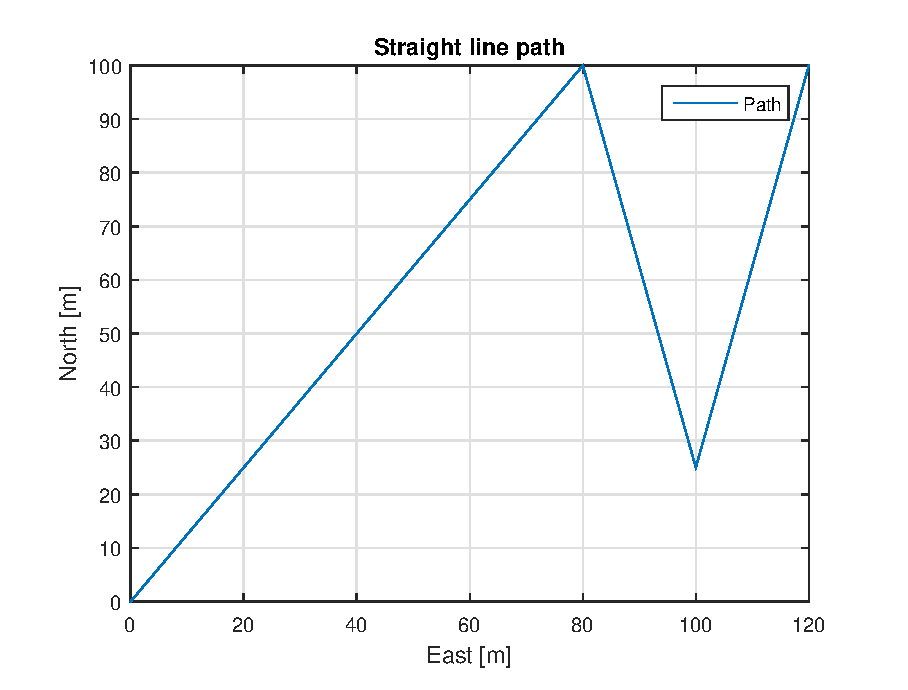
\includegraphics[width=0.7\textwidth]{figs/TheoryPlot/StraightLine.eps}
\end{figure}
The simplest for of creating a path is a straight line between two way-points. The advantage with a straight line is that it's easy for a guidance system to follow the line, however it will experience a jump in reference when transitioning to another straight line due to discontinuous tangential vector.
\section{Dubins path}\label{S:DubinsPath}
An alternative to a straight line path is a path constructed by straight lines and circle. Rudolf Dubin showed \citep{dubins1957curves} that the shortest possible path for a particle that moved with unit speed with maximum curvature would consist of three pieces. The path is considered as the shortest path from $P_s$ to $P_f$, however the curvature is discontinues, which gives a smoothness level of $G^1$ and $C^0$. 
Dubins path is the shortest path from from one way-point to the other which is continues. Dubins path can be created for a three dimensional case, however a simplification is made in which only a planar version of the Dubins path is examined. A Dubin path with fixed end orientation can be constructed in four different way.
\begin{table}[H]
\centering
\begin{adjustbox}{max width=\textwidth}
\begin{tabular}{ | l |}
\hline
Right to Right \\
Right to left \\
Left to Right \\
Left to left \\ \hline
\end{tabular}
\end{adjustbox}
\caption{Turning direction for Dubins path with fixed final orientation}
\label{Tb:DubinsTurningDirection}
\end{table}

Allowing the finish orientation to be free will add four more variants of the Dubins path.
The path consist of two arcs and a straight line. The straight line is tangential to both arcs. The start and end point of the straight line can be found with
\begin{subequations}
\begin{align}
& \alpha = \arcsin\big(\frac{\rho_f-\rho_s}{|c|}\big) \\
& \beta = \arctan\big(\frac{y_{cf}-y_{cs}}{x_{cf}-x_{cs}}\big)
\end{align}
\end{subequations}

\begin{table}[H]
\begin{center}
\begin{tabular}{ | l | | l |}
\hline
& \textbf{Turn angle} \\ \hline
$\phi_{right}$ & $\alpha + \beta + \frac{\pi}{2}$ \\
$\phi_{left}$ & $\beta - \alpha + \frac{3\pi}{2}$ \\ \hline
\end{tabular}
\end{center}
\end{table}

\begin{subequations}
\begin{align}
& x_{P_\chi} = x_{cs} + R_s\cos(\phi) \\
& y_{P_\chi} = x_{cs} + R_s\sin(\phi) \\
& x_{P_N} = x_{cf} + R_f\cos(\phi) \\
& y_{P_N} = x_{cf} + R_f\sin(\phi)
\end{align}
\end{subequations}
\begin{figure}[H]
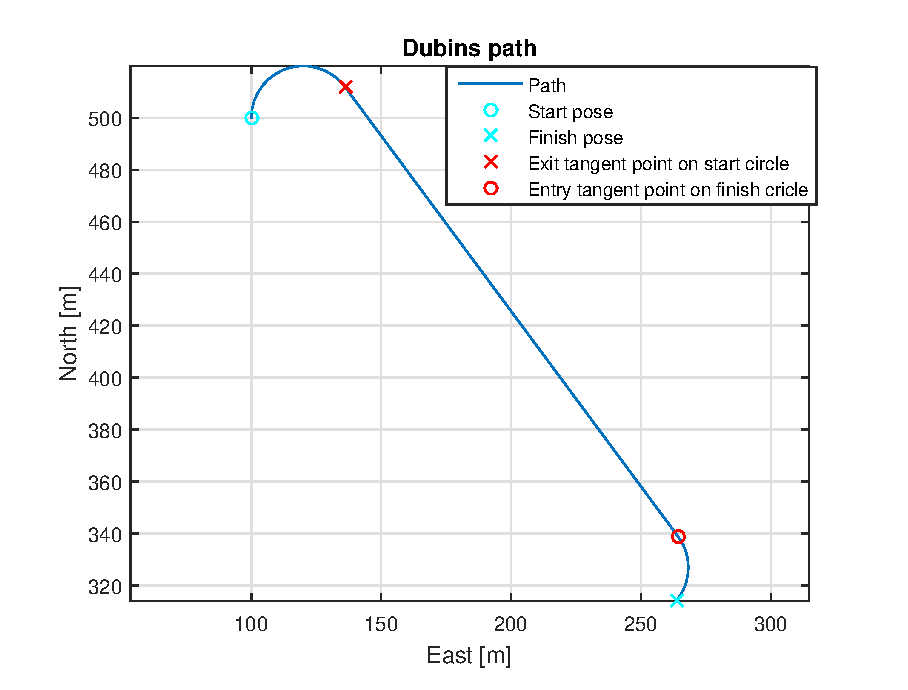
\includegraphics[width=0.7\textwidth]{figs/TheoryPlot/DubinsPath.eps}
\end{figure}
%\chapter{RTKGPS}
This chapter present some of the basic theory behind rtkgps.

When phase measurement is applied an important part. Integer ambiguity is the uncertainty of the number of whole cycles between the receiver and a satellite.


\section{Real time kinematic GPS}\label{ss:rtk-gps}
In \citep{misra2011global} section 7.2.2 \arcfull{rtk-gps} is defined as a rover that receive raw measurements from a reference receiver which is transmitted over a radio link, with a key feature that the rover is able to estimate the integer ambiguities while moving. The reference receiver is usually defined as a base station, and the integer ambiguity is the uncertainty of the number of whole phase cycles between the receiver and a satellite. With the measurements from the base station the rover is able to calculated the distance between itself and the base station, where the distance is referred to as a baseline. The length of the baseline affect the accuracy of the \gls{rtk-gps} solution, due to increased effect of atmospheric disturbance, which is further explain in \ref{Ss:Atmosphere}. However with a short baseline, e.g. $1-2 km$, the atmospheric condition can be considered equal for the base station and the rover, which keeps the solution  at centimetre level accuracy.

The ability for the rover to resolve the integer ambiguity is a key feature in \gls{rtk-gps}. A well used method was purposed in the article \citep{teunissen1994new} which decorrelate the integer ambiguities such that a efficient computation of the least square estimate can be performed. The search method is further explained in \citep{teunissen1995least}. A estimate of the integer ambiguity with sufficient high degree of certainty is referred to as a FIX solution, otherwise the solution is degraded to FLOAT where the integer ambiguity is allowed to be a decimal or a floating point number. When the solution is categorised as FIX the accuracy of the solution is considered on centimetre level, while with a FLOAT solution the accuracy is at a decimetre level.

\gls{rtk-gps} can either provide a kinematic setting or a moving baseline setting. The difference between the two is that in kinematic the base station has a known stationary position, while in moving baseline the base station position is unknown and allowed to move. The unknown base station position is calculated with a single receiver, with the accuracy that entails. Therefore the \gls{rtk-gps} system with a moving baseline configuration can never have better global accuracy then what it will get with a single receiver. The advantage with the moving baseline configuration is that \gls{rtk-gps} can be used to find the relative position between two dynamical system using \gls{gnss} in real time. This will be the case in automatic ship landing system, where the base station is on a ship, thus must be allowed to move. The advantage with kinematic mode is that it can give a more accurate position estimate, where the relative position of the rover can be given in either the \gls{ned} or \gls{enu} frame.

\begin{figure}[H]
	\centering
		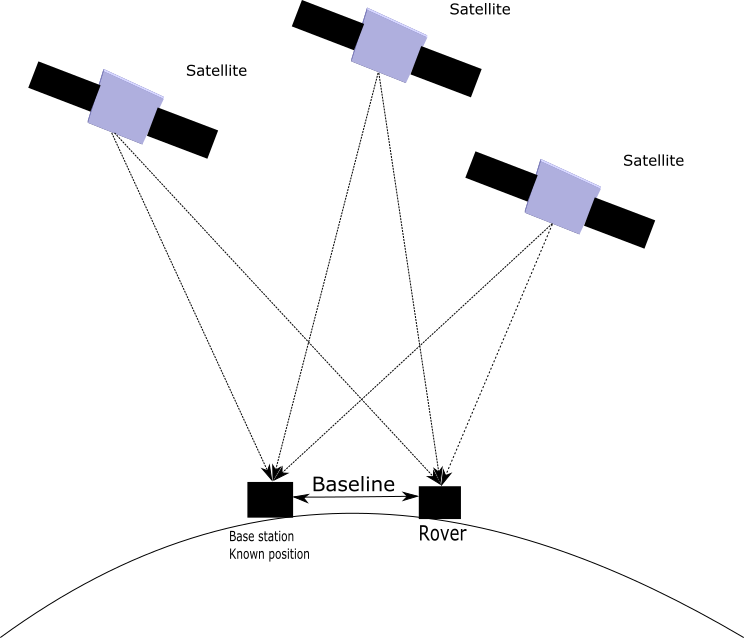
\includegraphics[width=0.7\textwidth]{figs/DGPS.png}
		\caption{Concept figure of \acrfull{dgps}}
		\label{figure:DGPS}
\end{figure}
\section{Error sources}
In order to get high accuracy in the position estimation the different error sources must be identified and removed if possible. This section will identify some of the most significant error sources that can affect the \gls{gnss} signal, and how to remove or mitigate them in the estimation.
\subsection{Clock error}
There is drift in both the satellite clock and the receiver clock. The atomic clock in the satellites makes the clock drift negligible from the user perspective. The receiver clock tend to drift, and if not taken into account will cause large deviations in the position estimate from the true position. This error is remove by including a fourth satellite in the position computation. The satellite clock error is given in the satellite message. 

\subsection{Ionospheric and tropospheric delays}\label{Ss:Atmosphere}
When the \gls{gps} signals travel though the atmosphere there will be a delay caused by the different atmospheric layers.
\subsubsection{Ionospheric delay}
Gas molecules in the ionosphere becomes ionized by the ultraviolet rays that is emitted by the sun, which release free electrons. These electron can influence electromagnetic wave propagation, such as \gls{gnss} signals. In \citep{vik2014integrated} section 3.5.1 it's stated that the delay caused by the ionosphere usually is in the order of $1-10 $meters. The error can be mitigated by using a double frequency receiver, or by applying a mathematical model to estimate the delay. Both those methods are with a single receiver, however by including a second receiver the \gls{gnss} solution system can assume that both receiver receive signal in the same epoch, which means that the signals have experienced the same delay.

\subsubsection{Tropospheric delay}
The tropospheric delay is a function of the local temperature, pressure and relative humidity. From \citep{vik2014integrated} section 3.5.1 the delay can vary from $2.4$ meters to $25$ meters depending on the elevation angle of the satellites. The error can be mitigated by applying a mathematical model to estimate the tropospheric delay, or by using a elevation mask can remove all satellites with a elevation angle bellow a certain threshold. Error caused by tropospheric delay can be removed in the same manners as ionospheric delay when using two or more receivers. 
\subsection{Ephemeris errors}
A satellite is not able to perfectly follow a given orbit, therefore there will be a deviation between satellite position given to the receiver and the true position of the satellite. This is called the ephemeris error. The true position of a satellite is monitored and corrected by the owner of the \gls{gnss} constellation, but error between each correction can be expected.
\subsection{Multipath}
One of the primary source of error in in a GNSS receiver is multipath. Multipath happens when the satellite signal is reflected by a nearby surface before if reach the \gls{gnss} antenna. The delay introduced in the signal can make the receiver believe that its position is several meters away form its true position. The easiest way to mitigated multipath is to place the antenna at a location with open skies, and no tall structures nearby.

Multipath error uncorrelated between receivers, thus the local receiver must be able to correct for multipath error locally.
\cleardoublepage
\chapter{Path and navigation}\label{CH:PathNavigation}
This chapter contain the system description of the landing plan generator and the navigation system.
\section{Landing plan}\label{Ch:LandingPlan}
The landing plan consist of two main parts, which the landing path and the approach path. The landing path is a straight line path orientated with respect to a reference position, which in this system is the position of the net. The approach path is design as a lateral Dubins path and a longitudinal straight line path, with the guaranty  that the \gls{uav} is able to enter the landing path at the correct height with the correct orientation.
\subsection{Landing Path}\label{SS:netApproach}
The landing path is inspired by the work done in \citep{Skulstad&Syversen} where waypoints was used to create a straight line path towards the net. This method proved successful, and thus this landing system continues on the work. The decent angle of the straight line path should be kept small to avoid build up in speed, however the trade off is that the start high in of the landing path must be above any obstacles that is around the landing area. A waypoint is here defined as:
\begin{equation}
\textbf{WPn} = \begin{bmatrix}
x \\
y \\
z
\end{bmatrix}
\end{equation}
where $x,y,z \in \Bbb R^3$. The straight line path is constructed relative to the net as shown in figure \ref{Fig:LandingPhase}, with way-points given as:
\begin{subequations}
\begin{align}
&\mathbf{WP4} = 
\begin{bmatrix}
-a0 \\
0 \\
h_{nc} + a1\tan(\gamma_n) 
\end{bmatrix}\\
&\mathbf{WP3} = 
\begin{bmatrix}
a1 \\
0 \\
h_{nc} - a1\tan(\gamma_n)
\end{bmatrix}\\
&\mathbf{WP2} = \mathbf{WP3} + 
\begin{bmatrix}
a2 \\
0 \\
-a2\tan(\gamma_l)
\end{bmatrix}\\
&\mathbf{WP1} = \mathbf{WP2} + 
\begin{bmatrix}
a3 \\
0 \\
0 \\
\end{bmatrix}
\end{align}
\end{subequations}
where the description of the parameters used is given in table \ref{Tb:Approach Parameters}. The net is placed between the fourth and third way points, in order for the fourth waypoint to be a aiming point for the \gls{uav} and avoid transitional behaviour before hitting the net.
\begin{table}[H]
\begin{center}
    \begin{tabular}{ | l | l |}
    \hline
    \textbf{Parameter} & \textbf{Description} \\ \hline
    $h_{nc}$ & The height from ground to the net center \\ \hline
    $a0$ & The distance behind the net \\ \hline
    $a1$ & The distance in front of the net \\ \hline
    $a2$ & The length of the glide slope \\ \hline
    $a3$ & The length of the approach towards the glide slope \\ \hline
    $\gamma_n$ & The net attack angle \\ \hline
    $\gamma_l$ & The landing glide slope angle \\ \hline
    \end{tabular}
\end{center}
\caption{Landing path parameters }
\label{Tb:Approach Parameters}
\end{table}
Continuing the waypoints are rotated into the NED frame by a rotation around the z-axes.
\begin{equation}
\mathbf{WP}^n = \mathbf{R}(\psi_{net})\mathbf{WP}^b
\end{equation}
were $\psi_{net}$ is the heading of the net, and $\mathbf{R}(\psi_{net})$ is the standard rotation matrix around the z-axis.
\begin{figure}
\def\svgwidth{\textwidth} % Defining the width since Inkscape hasn't done this yet in the .pdf_tex file
\input{InkFig/LandingPhase.pdf_tex}
\caption{The landing path}
\label{Fig:LandingPhase}
\end{figure}

\subsection{Approach path}\label{SS:LandingApproach}
The approach path is separated into two parts, which is a lateral and longitudinal path. The purpose of the path is to ensure that the \gls{uav} can enter the landing path at the correct height with the correct orientation from any initial position. The lateral and longitudinal paths are created separately 
\subsubsection{Lateral path}
The lateral path is designed as a Dubins path, with start pose, $P_s$, which is the pose where the landing plan generation request was made, and final pose, $P_f$, which is the start position of the landing path with the orientation towards the net. Dubins path was chosen due to its circular turns, simplistic design , and meet the requirement that the \gls{uav} enters the landing path with the correct orientation.

The lateral path is constructed with the equations presented in section \ref{S:DubinsPath}. The standard approach path is the shortest path of the four different rotation pairs given in table \ref{Tb:DubinsTurningDirection}, however when implemented there exits the option of manually setting the rotation direction for both circles. The shortest path is determined by calculating the length of each variants, where the shortest is chosen. The resulting the path is shown in figure \ref{Fig:LateralPath}.
\begin{figure}[H]
	\centering
		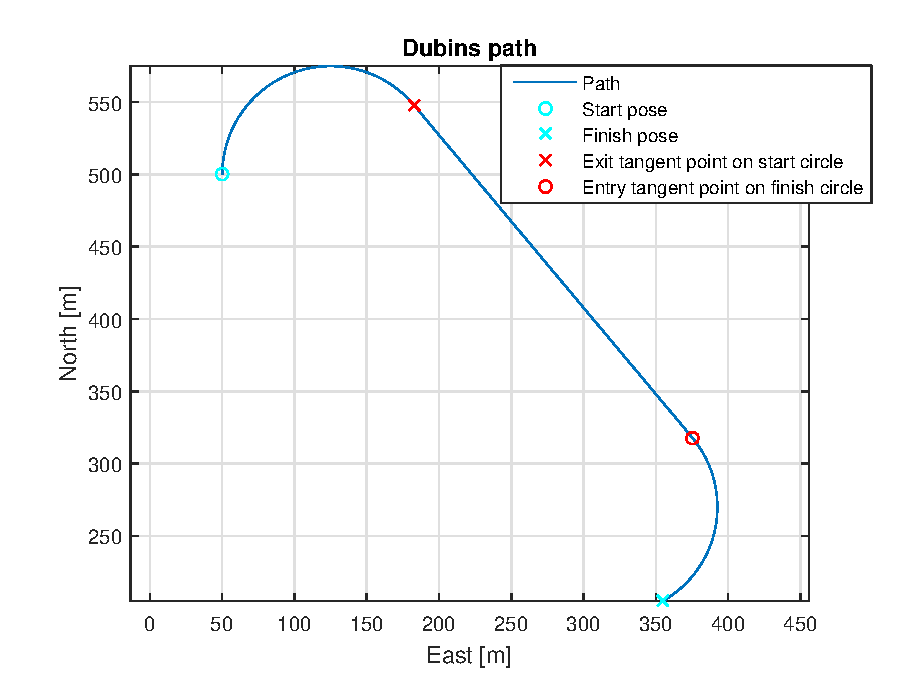
\includegraphics[width=1\textwidth]{figs/SysPlot/DubinsPath.eps}
		\caption{Lateral Dubins path}
		\label{Fig:LateralPath}
\end{figure}

The construction of the lateral path consists of two arc with a straight line between the arcs. The arcs are constructed by first finding the entry and exit angle with respect to the inertia frame, defined as $\psi_0$ and $\psi_1$ respectfully:
\begin{subequations}
\begin{align}
\psi_0 &= \begin{cases}
\atan2(Y_s-Y_{cs},X_s-X_{cs}) & \text{if start circle} \\
\atan2(Y_{P_N}-Y_{cf},X_{P_N}-X_{cf}) & \text{otherwise}
\end{cases}\\
\psi_1 &= \begin{cases}
\atan2(Y_{P_\chi}-Y_{cs},X_{P_{\chi}}-X_{cs}) & \text{if start circle} \\
\atan2(Y_{f}-Y_{cf},X_{f}-X_{cf}) & \text{otherwise}
\end{cases}
\end{align}
\end{subequations}
Continuing the turn angle must be defined, which is the difference between $\psi_1$ and $\psi_0$. However the periodic behaviour of the unit circle must be respected, in addition to the rotation direction. The maximum turning angle becomes:
\begin{equation}
\psi_{max} = \begin{cases}
-|\psi_1 - \psi_0| & \text{if counter clockwise rotation and } \psi_1 - \psi_0 \leq 0 \\
-(2\pi - |\psi_1-\psi_0|) & \text{ if counter clockwise rotation and } \psi_1 - \psi_0 > 0 \\
|\psi_1 - \psi_0| & \text{if clockwise rotation and } \psi_1 - \psi_0 \geq 0 \\
(2\pi - |\psi_1-\psi_0|) & \text{ if clockwise rotation and } \psi_1 - \psi_0 < 0
\end{cases}
\end{equation}
where $|\psi_1-\psi_0| \in(-\pi,\pi]$. From the maximum turning angle the angle step and number of angle segments in the arc can be determined:
\begin{subequations}
\begin{align}
h &= \text{sign}\frac{d_{arc}}{R} \\
N &= \ceil[\Bigg]{\frac{\text{sign}(\psi_{max})\psi_{max}}{|h|}} + 1
\end{align}
\end{subequations}
where $h$ is arc angle step and $N$ the total number of steps in the arc. The step angle must have the same sign as $\psi_{max}$ to ensure the correct rotation direction. Continuing the heading function $\psi(\varpi)$ can be defined as:
\begin{equation}
\psi(\varpi) = \begin{cases}
\psi_{max} & \varpi = N-1 \\
\varpi h & \text{otherwise}
\end{cases}
\end{equation}
where $\varpi = 1,...,N-1$. Finally the arc path can be defined as:
\begin{equation}
\mathbf{p}(\varpi) = \begin{bmatrix}
\mathbf{O}_c \\
\end{bmatrix} + R\begin{bmatrix}
\cos(\psi_0 + \psi(\varpi)) \\
\sin(\psi_0 + \psi(\varpi)) \\
\end{bmatrix}
\end{equation}
A summary of the lateral path is:
\begin{equation}
\mathbf{p}(i) = \begin{cases}
\begin{bmatrix}
\mathbf{O}_{cs} \\
\end{bmatrix} + R_s\begin{bmatrix}
\cos(\psi_{0} + \psi(\varpi)) \\
\sin(\psi_{0} + \psi(\varpi)) \\
\end{bmatrix} & \text{Start circle} \\
\begin{bmatrix}
\mathbf{O}_{cf} \\
\end{bmatrix} + R_f\begin{bmatrix}
\cos(\psi_{0} + \psi(\varpi)) \\
\sin(\psi_{0} + \psi(\varpi)) \\
\end{bmatrix} & \text{Finish circle}
\end{cases}
\end{equation}
where $i \in [1,...,N_s + N_f]$ with $N_s$ and $N_f$ as the number of segments in the start and finish circle respectfully.
\subsubsection{Longitudinal path}
The longitudinal path is designed as a straight line path along the lateral path, which fused together with the lateral path forms a spiral path towards the landing path. The approach path hold a constant decent angle until the correct height is reached, which is defined as the start height for the landing path. The approach decent angle is then adjusted in order for the correct height to be reach. The approach decent angle is defined as:
\begin{equation}
\gamma_d = \begin{cases}
\atan2(\Delta z,||\mathbf{p}(i+1)-\mathbf{p}(i)||_2) & \text{if } \atan2(\Delta z,||\mathbf{p}(i+1)-\mathbf{p}(i)||_2)\leq \gamma_{d_{Max}} \\
\gamma_{d_{Max}}										& \text{otherwise}
\end{cases}
\end{equation}
where $\gamma_{d_{Max}}$ is the maximum decent angle for the approach path, and $\Delta z$ is defined as:
\begin{equation}
\Delta z = z_d-z(i)
\end{equation}
where $z_d$ is the $z$ component in $WP1$. Continuing the longitudinal path is given as:
\begin{equation}
\mathbf{r}(i+1) = \begin{bmatrix}
\mathbf{p}(i) \\
||\mathbf{p}(i+1)-\mathbf{p}(i)||_2\tan(\gamma_d)
\end{bmatrix}
\end{equation}
where $\mathbf{r}(i)$ is the landing path and 
$p = \begin{bmatrix}
x(i) & y(i)
\end{bmatrix}^T$ is the lateral path. The resulting height profile of the approach path is shown in figure \ref{Fig:HeightProfile}.
\begin{figure}[H]
	\centering
		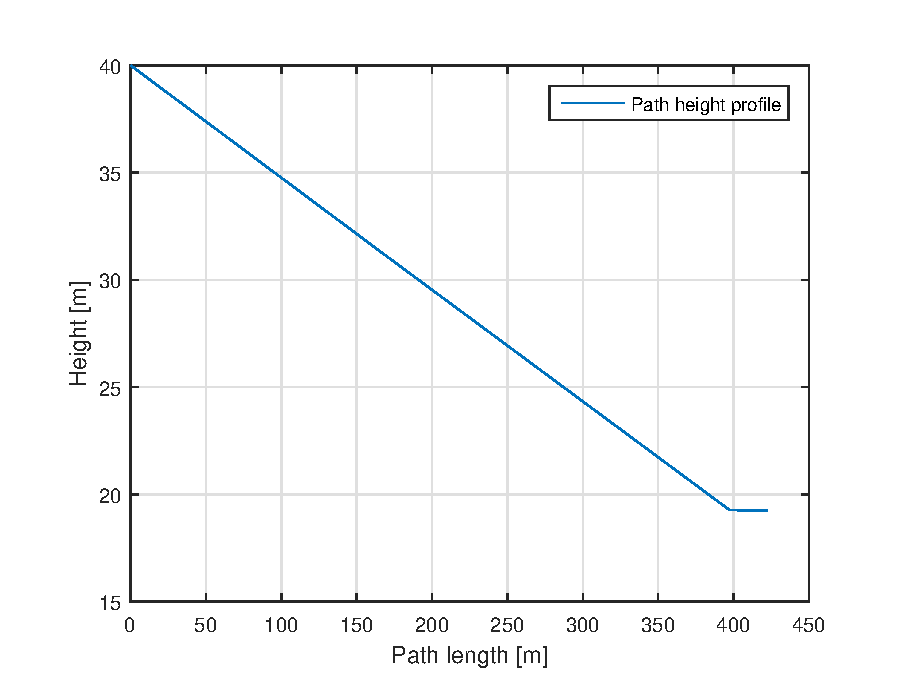
\includegraphics[width=1\textwidth]{figs/SysPlot/heightProfile.eps}
		\caption{Height profile of the landing path}
		\label{Fig:HeightProfile}
\end{figure}
\paragraph{Spiral path}\label{pp:SpiralPath}
In the case where the approach path has yet to reach the correct heigh at the end of the combined lateral and longitudinal path a new spiral path is created in order for the approach path to reach the height of the landing path. The spiral path is designed to have the same turning radius, turning direction and decent angle as the approach path. The longitudinal path continues along the spiral until the correct height can be reached with and decent angle equal or less then $\gamma_{d_{Max}}$. Continuing an arc is created such that the path ends with the correct heading. The arc has the same rotation direction as the lateral path, with start point where the correct height was reached and end point of the start of the landing path. The complete approach path combined with the landing path is shown in figure \ref{Fig:LateralPath}.
\begin{figure}[H]
	\centering
		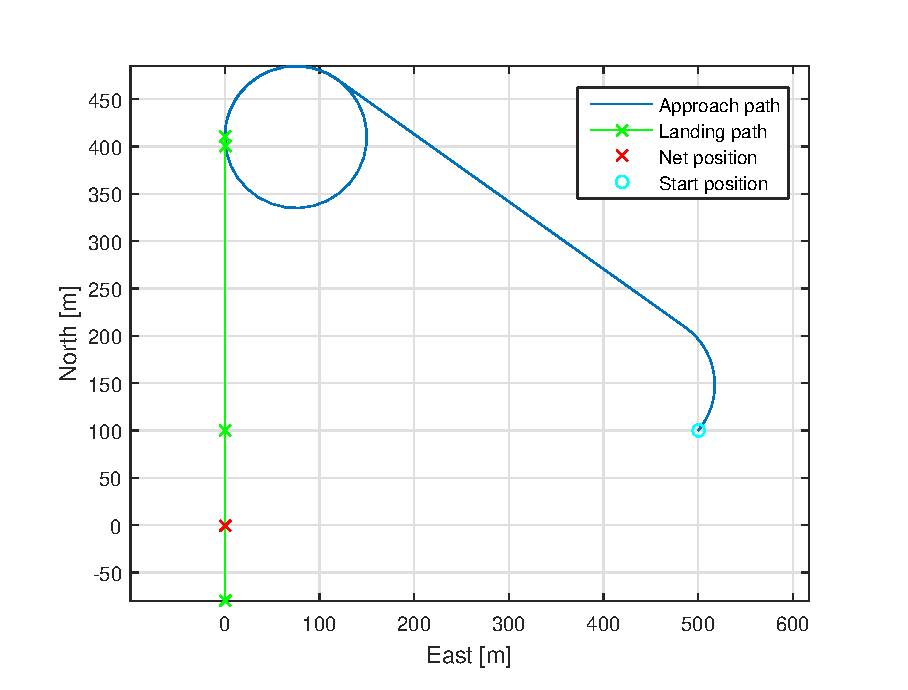
\includegraphics[scale=0.7]{figs/SysPlot/LandingPath.eps}
		\caption{Approach path connected to the landing path}
		\label{Fig:LandingPath}
\end{figure}
\section{Navigation system}
The navigation system consist of two position and velocity measurement system, where one is a high accurate positioning system and the other a reliable backup system. The high accurate positioning system apply \gls{rtk-gnss}, which is able to provide high accurate position solution. The backup positioning system consist of a standard package of standalone \gls{gps} and Inertial Measurement Unit (IMU) together with a Kalman filter, which is a proven reliable system in Ardupilot together with a Pixhawk. Ardupilot and Pixhawk are explained further in section \ref{ss:ardupilot} and section \ref{ss:Pixhawk}. However the \gls{rtk-gnss} is subject to drop out, which must be handled by the navigation system. A state machine has been created to handle the state switching between \gls{rtk-gps} and the external navigation data, which is navigation data from the Pixhawk. A short drop out of the \gls{rtk-gnss} could be resolved by fusing data from the external navigation source together with previous position solutions from the \gls{rtk-gnss}, and create a compensator for the external navigation system. The compensator can then be used to achieve the same accuracy as the \gls{rtk-gnss} for a short period.
\subsection{Position estimation RTK-GPS}\label{ss:rtk-gps}
\acrfull{rtk-gnss} is in \citep{misra2011global} section 7.2.2 defined as a rover that receive raw \gls{gnss} measurements from a reference receiver which is transmitted over a radio link. A key feature with \gls{rtk-gnss} is that the rover is able to estimate the integer ambiguities while moving. The reference receiver is usually defined as a base station, and the integer ambiguity is the uncertainty of the number of whole phase cycles between the receiver and a satellite. With the measurements from the base station the rover is able to calculated the distance between itself and the base station, where the distance is referred to as a baseline. The length of the baseline affect the accuracy of the \gls{rtk-gnss} solution, due to increased effect of atmospheric disturbance, which is further explain in \ref{Ss:Atmosphere}. However with a short baseline, e.g. $1-2 km$, the atmospheric condition can be considered equal for the base station and the rover, which keeps the solution  at centimetre level accuracy. The concept of \gls{rtk-gnss} is depicted in figure \ref{figure:RTK}.
\begin{figure}[H]
	\centering
		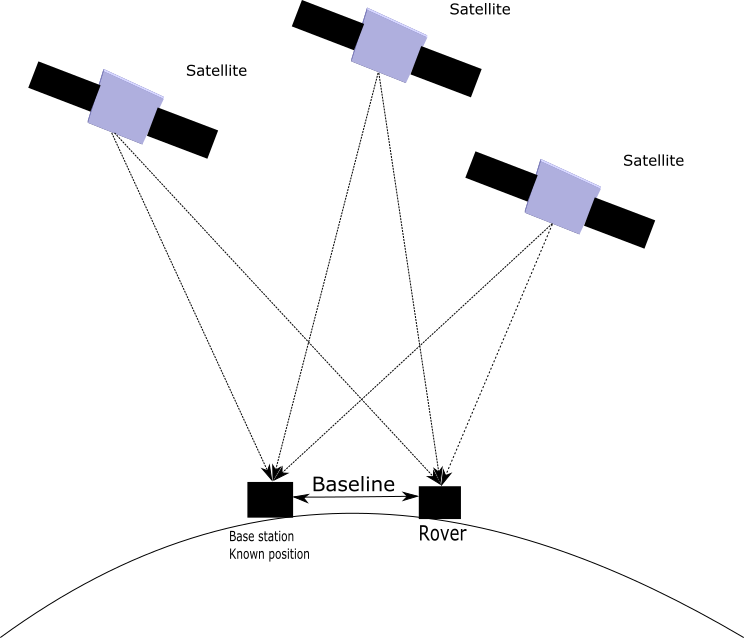
\includegraphics[width=0.7\textwidth]{figs/DGPS.png}
		\caption{Concept figure of \acrfull{rtk-gnss}}
		\label{figure:RTK}
\end{figure}
The ability for the rover to resolve the integer ambiguity is a key feature in \gls{rtk-gnss}. A well used method was purposed in the article \citep{teunissen1994new} which decorrelate the integer ambiguities such that a efficient computation of the least square estimate can be performed. The search method is further explained in \citep{teunissen1995least}. A estimate of the integer ambiguity with sufficient high degree of certainty is referred to as a FIX solution, otherwise the solution is degraded to FLOAT where the integer ambiguity is allowed to be a decimal or a floating point number. When the solution is categorised as FIX the accuracy of the solution is considered on centimetre level, while with a FLOAT solution the accuracy is at a decimetre level. However when a FIX solution is lost, the solution accuracy will not imminently degrade to decimetre level.

In \gls{rtk-gnss} the position of the base station must be resolved. This can be achieved by either knowing the position beforehand, which is defined as a kinematic configuration. If the base station position is unknown the \gls{rtk-gnss} solver calculates the position on the fly, which is defined as a moving baseline configuration. The unknown position is then calculated as a standalone \gls{gnss} receiver, with the accuracy that entails. Therefore the \gls{rtk-gps} system with a moving baseline configuration can never have better global accuracy then what it will get with a single receiver. The advantage with the moving baseline configuration is that the base station is allowed to moved, and with \gls{rtk-gnss} the relative position between the rover and base station can be determined in real time. The advantage with kinematic mode is that it can give a more accurate position estimate, however this require that the base station is known and stationary.
\subsubsection{Error sources}
In order to get high accuracy in the position estimation the different error sources must be identified and removed if possible. This section will identify some of the most significant error sources that can affect the \gls{gnss} signal, and how to remove or mitigate them in the estimation.
\paragraph{Clock error}
There is drift in both the satellite clock and the receiver clock \citep{misra2011global}. The atomic clock in the satellites makes the clock drift negligible from the user perspective. The receiver clock tend to drift, and if not taken into account will cause large deviations in the position estimate from the true position. This error is remove by including a fourth satellite in the position computation. The satellite clock error is given in the satellite message.
\paragraph{Ionospheric and tropospheric delays}\label{Ss:Atmosphere}
When the \gls{gps} signals travel though the atmosphere there will be a delay caused by the different atmospheric layers \citep{misra2011global}. The atmosphere change the velocity of wave propagation for the radio signal, which results in altered transit time of the signal.
\paragraph{Ionospheric delay}
Gas molecules in the ionosphere becomes ionized by the ultraviolet rays that is emitted by the sun, which release free electrons. These electron can influence electromagnetic wave propagation, such as \gls{gnss} signals. In \citep{vik2014integrated} section 3.5.1 it's stated that the delay caused by the ionosphere usually is in the order of $1-10 $meters. The error can be mitigated by using a double frequency receiver, or by applying a mathematical model to estimate the delay. Both those methods are with a single receiver, however by including a second receiver in a network, e.g. \gls{rtk-gps}, the \gls{gnss} solution system can assume that both receiver receive signal in the same epoch, which means that the signals have experienced the same delay. The rover is then able to remove the error induced from ionospheric disturbance.
\paragraph{Tropospheric delay}
The tropospheric delay is a function of the local temperature, pressure and relative humidity. The effect of tropospheric delay can  vary from $2.4$ meters to $25$ meters depending on the elevation angle of the satellites,\citep{vik2014integrated} section 3.5.1. The error can be mitigated by applying a mathematical model to estimate the tropospheric delay, or by using a elevation mask can remove all satellites with a elevation angle bellow a certain threshold. Similar to ionospheric delay, tropospheric delay can be removed when using two receivers in a network by assuming that the single received by both receivers has experienced the same delay. 

\paragraph{Multipath}
One of the primary source of error in in a \gls{gnss} receiver is multipath \citep{misra2011global}. Multipath happens when the satellite signal is reflected by a nearby surface before if reach the \gls{gnss} antenna. The delay introduced in the signal can make the receiver believe that its position is several meters away form its true position. The easiest way to mitigated multipath is to place the antenna at a location with open skies, with no tall structures nearby. The effect can also be mitigated by choosing a antenna with good multipath rejection capability.

Multipath error uncorrelated between receivers, thus the local receiver must be able to correct for multipath error locally.

\subsection{Navigation state control system}\label{S:NavState}
The navigation state control system manage the current state of the navigation system, which controls the \gls{rtk-gnss} usage and is responsible for dispatching the current state of the \gls{uav} to the rest of the DUNE system. A state diagram of the navigation state control system is shown in figure \ref{Fig:NavState}, which included trigger event on the edges and entry actions when entering a new state. The entry actions ensure that only functionality that is connected to the current state is active, and that monitors are updated with the state switch. The navigation state control system is designed to function without \gls{rtk-gnss} available, which makes the navigation system independent from the \gls{rtk-gnss} system. This is a requirement for the navigation system since it should function in a \gls{uav} where \gls{rtk-gnss} is not present.

In order for the navigation system to switch state into "Rtk ready" the \gls{rtk-gps} message must be considered valid, which is defined in section \ref{ss:RTK-GPS system}. In addition the \gls{rtk-gps} solution type must be FIX for $x$ seconds such that the \gls{rtk-gnss} solution can be considered highly accurate. For the navigation state control system to switch to \gls{rtk-gnss}, the user has to enabled it from the command and control software used to monitor the \gls{uav}. In the case where a loss of \gls{rtk-gnss} is experienced the short \gls{rtk-gnss} compensator will be enable to prevent the loss of \gls{rtk-gnss} accuracy, thus prolonging the availability of the \gls{rtk-gnss}. This state will be further explained in section \ref{ss:ShortLoss}. A summary of the states in the navigation state control system is given in table \ref{Tb:StateDescription}.
\begin{figure}[H]
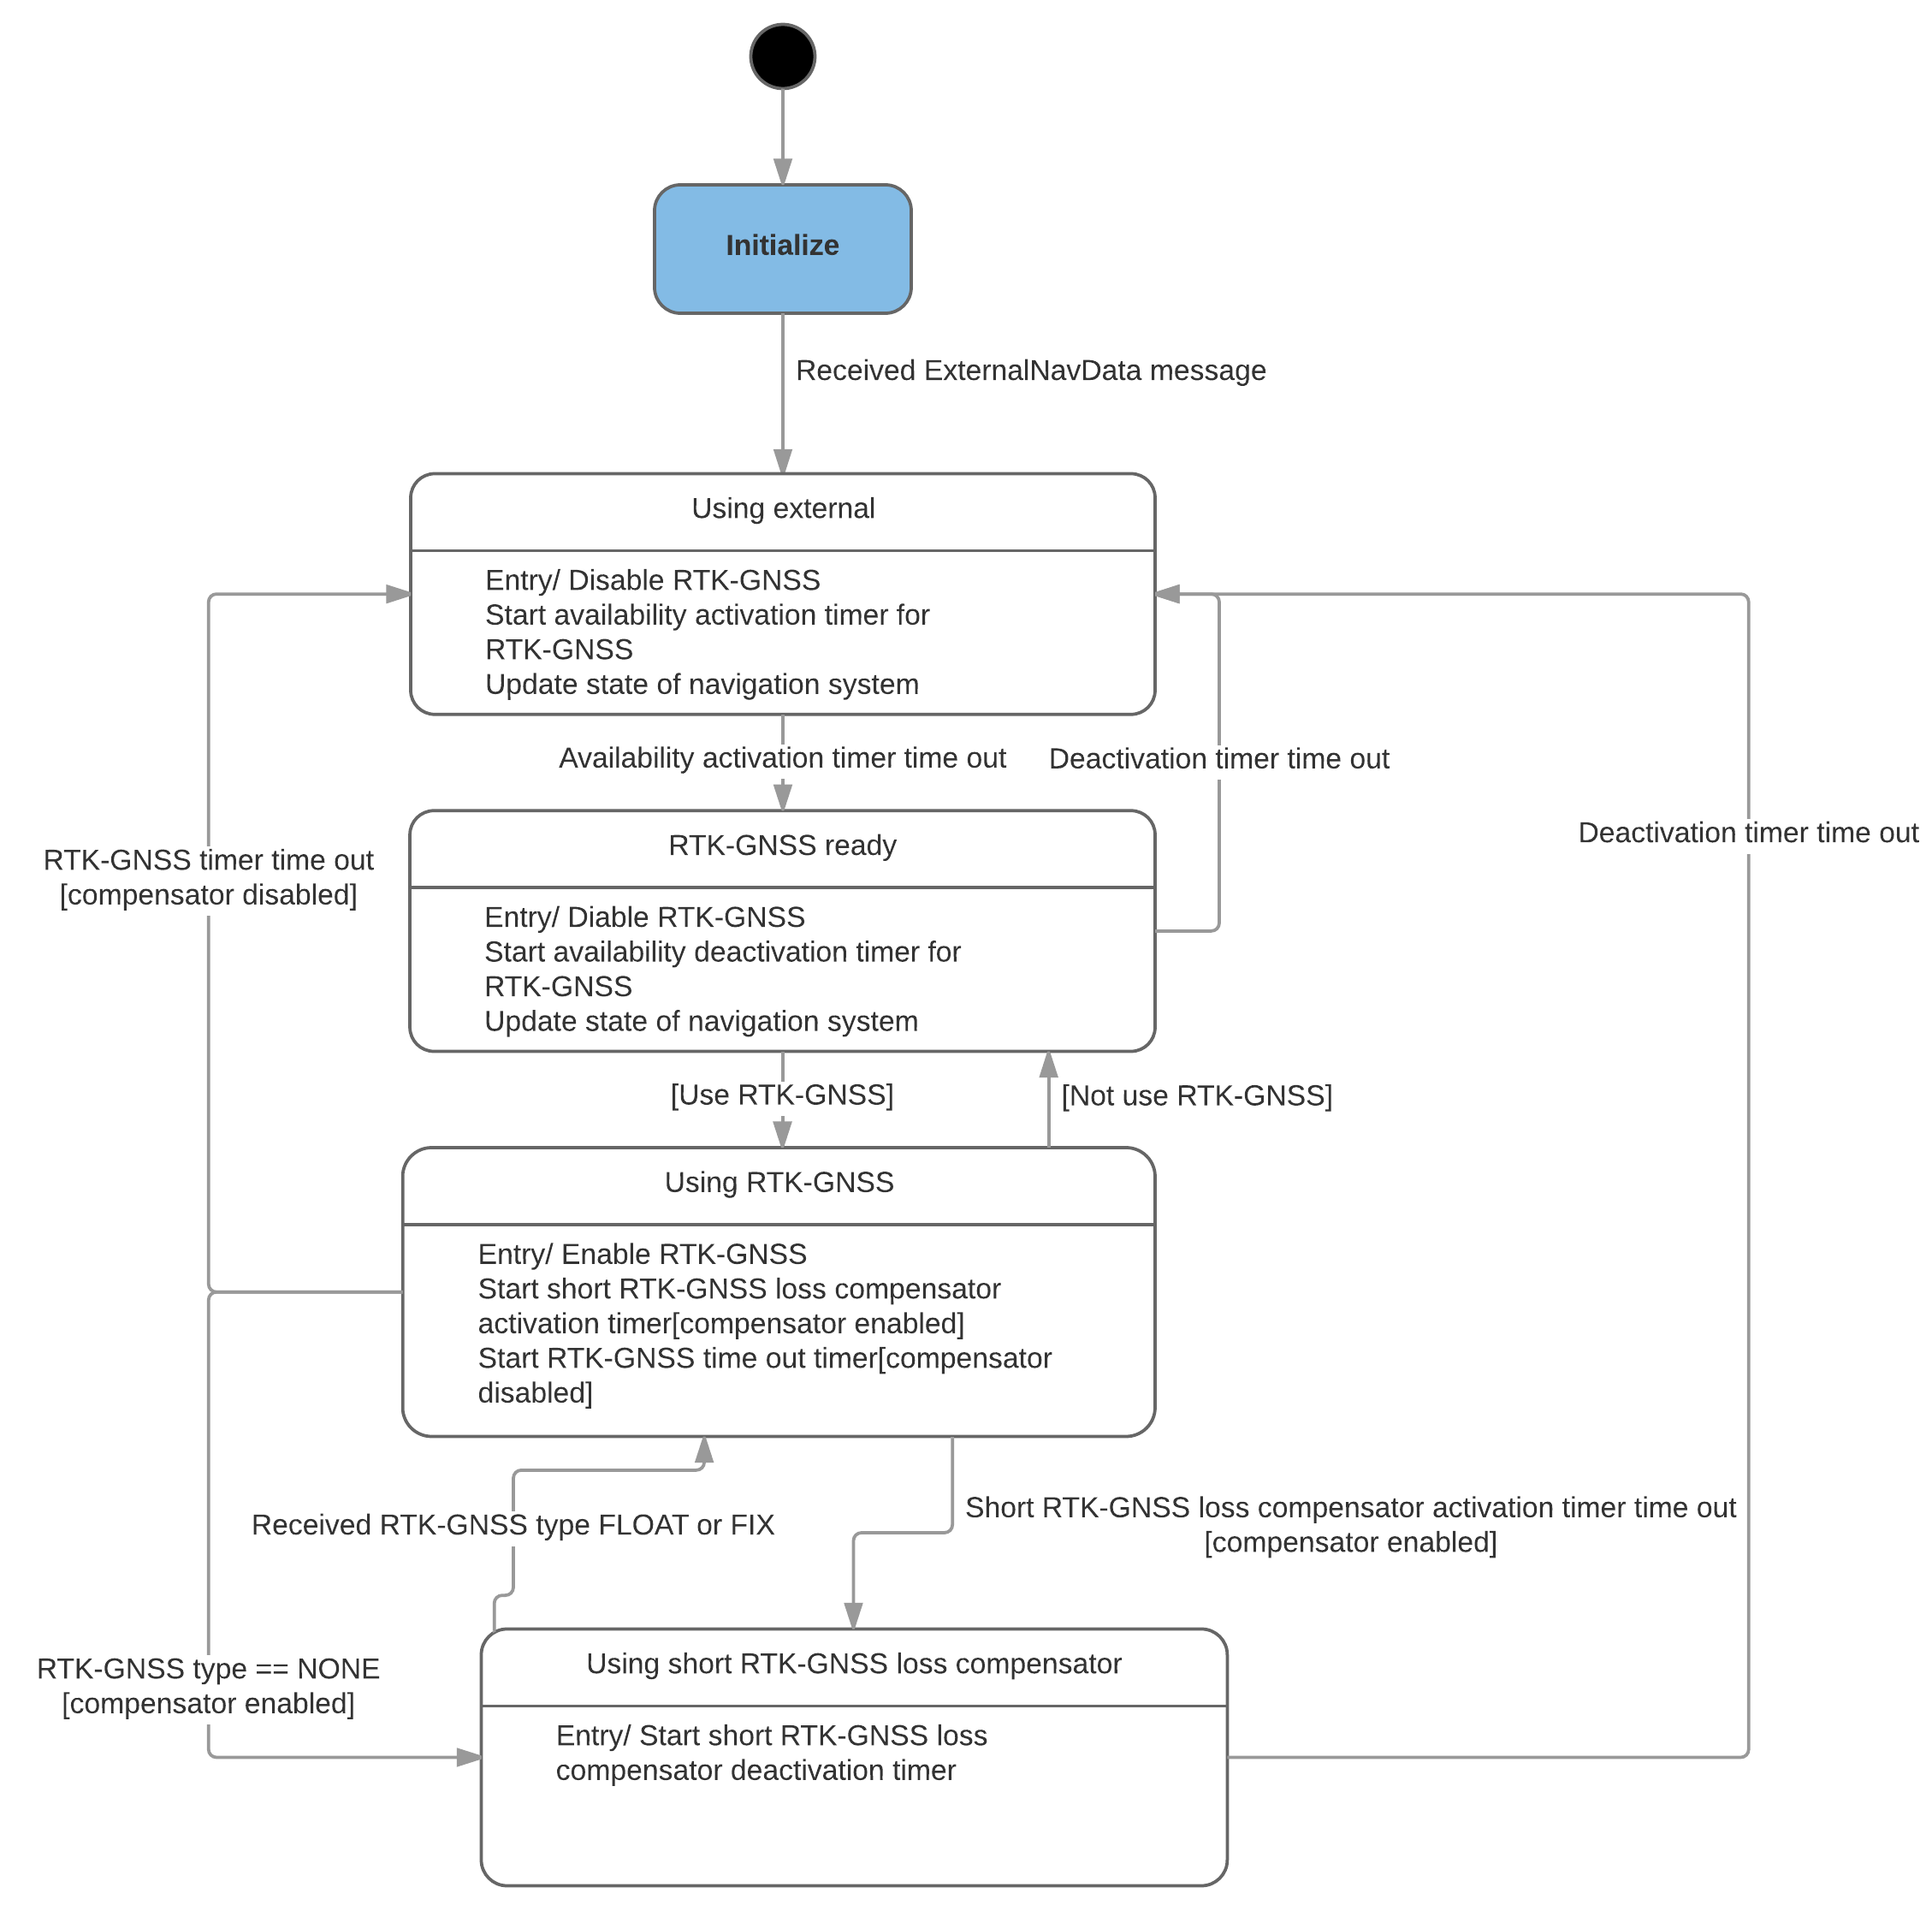
\includegraphics[scale=0.18]{figs/NavigationStateControl.png}
\caption{State machine in the DUNE Navigation task}
\label{Fig:NavState}
\end{figure}
\begin{table}[H]
\begin{tabular}{ | p{3cm} | p{8cm} |}
	\hline 
	\textbf{State}						& \textbf{Description} \\ \hline
	Initialize							& The task starting up\\ \hline
	Using external						& The navigation task apply the external navigation source in the state message\\ \hline
	\gls{rtk-gnss} ready							& The \gls{rtk-gnss} is ready for use, however the external navigation source is still used\\ \hline
	Using \gls{rtk-gnss}							& The navigation task apply the \gls{rtk-gnss} in the state message\\ \hline
	Using short \gls{rtk-gnss} loss compensator	& The navigation task apply the external navigation source with a compensation term to reduce the effect of \gls{rtk-gnss} loss. \\ \hline
\end{tabular}
\caption{States in the navigation system with description}
\label{Tb:StateDescription}
\end{table}
\subsubsection{Short loss of \gls{rtk-gnss}}\label{ss:ShortLoss}
In order for the navigation system to handle short loss of \gls{rtk-gps} a short loss \gls{rtk-gps} system is presented. The compensator is based on that the position solution from the external navigation system is almost constant with respect to the \gls{rtk-gps} solution. As seen in figure \ref{Fig:RTKExternal} the position of the \gls{rtk-gnss} and the external navigation system remain  close to each other, given that the \gls{rtk-gnss} has a FIX solution. 
\begin{figure}[H]
\centering
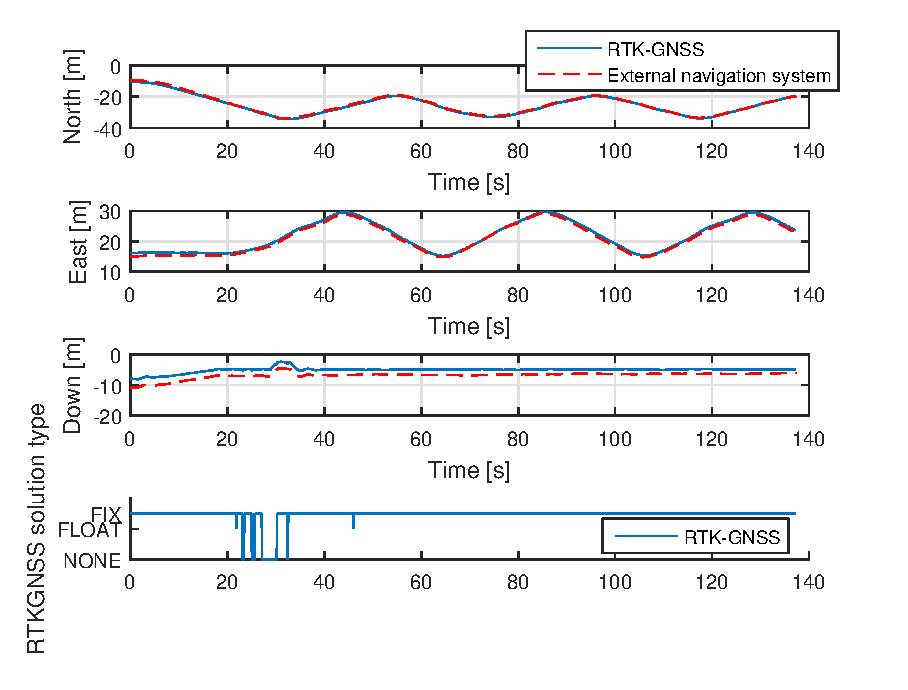
\includegraphics[scale=0.6]{figs/Experiment/RtkExternal.eps}
\caption{Plot where the \gls{rtk-gnss} solution is displayed together with the position solution from the external navigation system, include the solution type of the \gls{rtk-gnss} system.}
\label{Fig:RTKExternal}
\end{figure}
The slow moving difference between the \gls{rtk-gnss} and external navigation system position solution is confirmed in figure \ref{Fig:RtkExtDiff}.
\begin{figure}[H]
\centering
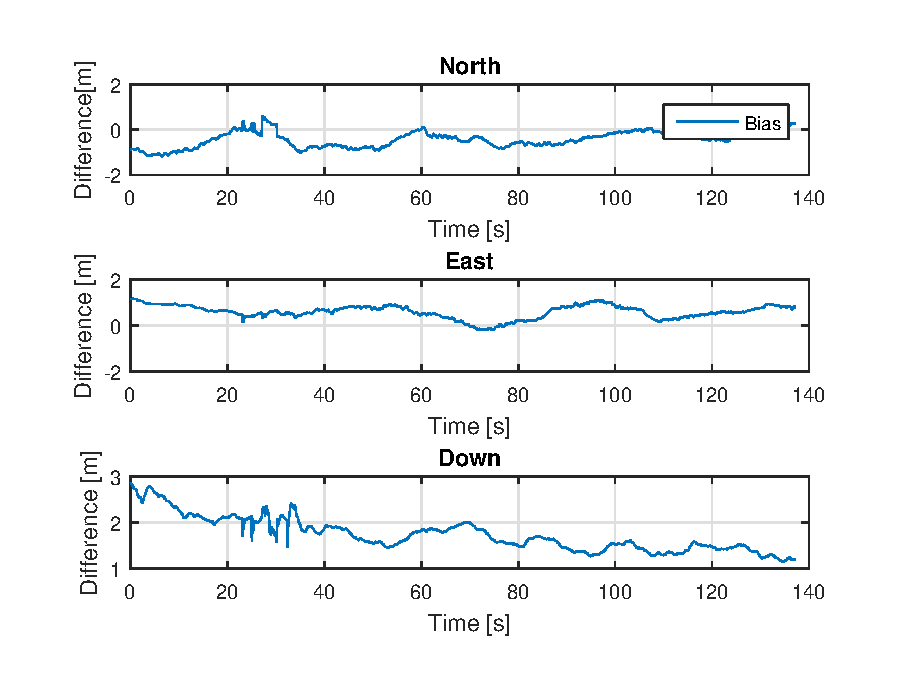
\includegraphics[scale=0.6]{figs/Experiment/biasShow.eps}
\caption{The difference between the \gls{rtk-gnss} solution and the external navigation system position solution}
\label{Fig:RtkExtDiff}
\end{figure}
Therefore the average difference between the \gls{rtk-gnss} position solution and the external navigation system should be able to move the external navigation position solution closer to the \gls{rtk-gps} position solution. The short loss compensator is given as:
\begin{align}
\mathbf{e}(n) &= \mathbf{p}_1(n) - \mathbf{p}_2(n)\\
\mathbf{\delta} &= \frac{1}{N}\sum_{n=0}^N(\mathbf{e}(n))
\end{align}
where $\mathbf{p}_1(n)$ and $\mathbf{p}_2(n)$ is the position solution sample for the \gls{rtk-gnss} system and the external navigation system respectfully. $N$ is the total number of samples with $n\in [0,N-1]$ as the counting variable. Adding $\mathbf{\delta}$ to the external navigation position with the assumption of slow varying bias between the two position solution gives:
\begin{equation}
\mathbf{p}_2(t) + \mathbf{\delta} \rightarrow \mathbf{p}_1(t)
\end{equation}
where $\mathbf{p}_1(t)$ and $\mathbf{p}_2(t)$ is the current position solution for the \gls{rtk-gnss} system and the external navigation system respectfully. The short loss \gls{rtk-gnss} compensator will trigger if there is a delay in the \gls{rtk-gnss} system, or a temporary drop out occur. The output frequency of the short loss compensator is set to be the same as the \gls{rtk-gnss} system, which is estimate by comparing the time each \gls{rtk-gnss} message is dispatched. This results in prolonging the time where the \gls{rtk-gnss} is available for the navigation system, and will ensure that the navigation system outputs at a stable frequency. The goal with the compensator is to prevent mission abortion, and make the \gls{rtk-gnss} system more robust.
\section{Summary}
This chapter has presented a system description of both a landing plan generator and a navigation system with robust \gls{rtk-gnss}. The landing plan presented is separated into two parts, which is the landing path and the approach path. The landing path is a straight line path towards the net, whereas the approach path is a combination of Dubins path in the lateral plane and straight line path in the longitudinal plane. The approach path is designed to guaranty that \gls{uav} has a flyable path which enable the \gls{uav} to enter the landing path at the correct height with the correct orientation from any initial position.

The \gls{uav} navigation system has been design with a navigation state control system, which is used to control the current state of the source of the navigation data. Currently the different navigation source available to the \gls{uav} is a external navigation system and a \gls{rtk-gnss} system. In order to prolong the availability of the \gls{rtk-gnss} during short drop outs a short \gls{rtk-gnss} loss compensator system is presented, which is used to compensate the external navigation system position solution in order for the \gls{uav} navigation system to keep the a \gls{rtk-gnss} accuracy level during a \gls{rtk-gnss} drop out.
\chapter{Software}
This chapter contain the software that is used for developing and testing the autonomous landing system for uav. 

The software that is mainly used in the uav system is based on a open-source software toolchain developed by the Underwater System and Technology Laboratory (LSTS). The toolchain supports air and ocean vehicle systems. The different components in the toolchain is IMC, DUNE, NEPTUS and Glued, which will be presented in later in this chapter. 

The rtkgps solution in the system is calculated in the open-source software RtkLib \citep{takasu2009development}. The desceription of the program is given in section \ref{s:Rtklib}.

The low level control system in the uav is controlled by Ardupilot, which is a 
\section{LSTS toolchain}
The software that the system is based on was developed by the Underwater Systems and Technology Laboratory (LSTS), which is called the LSTS toolchain \citep{pinto2013lsts}. The toolchain was developed for support of networked heterogeneous air and ocean vehicle systems. The toolchain supports interactions over wireless network, and is supports interaction with different system responseable for the low end control. The toolchain contain four different modules, namely \gls{imc}, DUNE, NEPTUS and Glued.
\subsection{IMC}
\gls{imc} \citep{martins2009imc} is design to enable interconnections between systems of vehicles, sensors and human operators, which enable the pursuit of common goal by cooperatively exchange real-time information about the environment and updated objectives. The message protocol is oriented around the message, which abstracts hardware and communication heterogeneity with a provided shared set of messages that can be serialized and transferred over different means. The \gls{imc} protocol is defined in a single eXtensible Markup Language (XML) document, which simplify the definition of exiting messages and the creation of new messages. A single XML document ease communication between two node when both node use the same document for message definition. 
\subsection{Dune}
DUNE (DUNE Uniform Navigation Environment) is a runtime environment for unmanned systems on-board software written in C++. DUNE is capable to interact with sensors, payload and actuators, in addition to communication, navigation, control, manoeuvring, plan execution and vehicle supervision. The software separate operations into different task that each has there own thread of execution. DUNE apply a message bus that is responsible for forwarding \gls{imc} message from the producer to all registered receivers, which is the only way different DUNE tasks is communicating. 

A DUNE task is enabled through a configuration file, where the user can choose in which profile the task should be enabled in. The different profile configuration in DUNE allows for testing the same system used in a hardware setting with a simulator.
\subsection{Neptus}
Neptus is a Command and Control software which is used to command and monitor unmanned systems that is written in Java. Neptus is able to provide coherent visual interface to command despite the heterogeneity in the controlled system that it is interacting with.  This allow the operator to command and control unmanned system without the need to dwell into specific command and control software in the unmanned system. The main communication channel for Neptus is \gls{imc}, which makes it interoperable with DUNE or other \gls{imc}- based peer.

Neptus is able to do MRA (Mission Review and Analysis) after a mission is finished. In the MRA phase Neptus analyse the \gls{imc} logs that is collected by e.g. DUNE, such that the result from a completed mission can be presented. In addition Neptus mission review is able to create output files of the log that can be analysed in third party software like Matlab.
\subsection{Glued}
Glued is a minimal Linux operating system distribution, and design with embedded system in mind. It is platform independent, easy to configure and contain only the necessary packages to run on a embedded system. This makes GLUED a light and fast distribution, which is ideal for a on-board operating system for a unmanned system where payload size is normally limited. GLUED is configured through a single configuration file that which can be created for a specific system.
\section{RTKLIB}\label{ss:Rtklib}
\acrfull{rtklib}\citep{takasu2009development} is a open source program package for standard and precise positioning with \gls{gnss} developed by T. Takasu. \gls{rtklib} can be configured to apply \gls{rtk-gps}, such that raw \gls{gnss} data is used estimate the relative position of the rover with respect to the base station in real time. Figure \ref{figure:RTKLIB_STRUCTURE} shows how \gls{rtklib} can be used in a \gls{rtk-gps} mode. The two main modules here is str2str and rtkrcv. Both will be explained more closely in the following sections. The version of \gls{rtklib} used in this thesis is \gls{rtklib}2.4.2 \citep{Rtklib242}.
\begin{figure}[H]
	\centering
		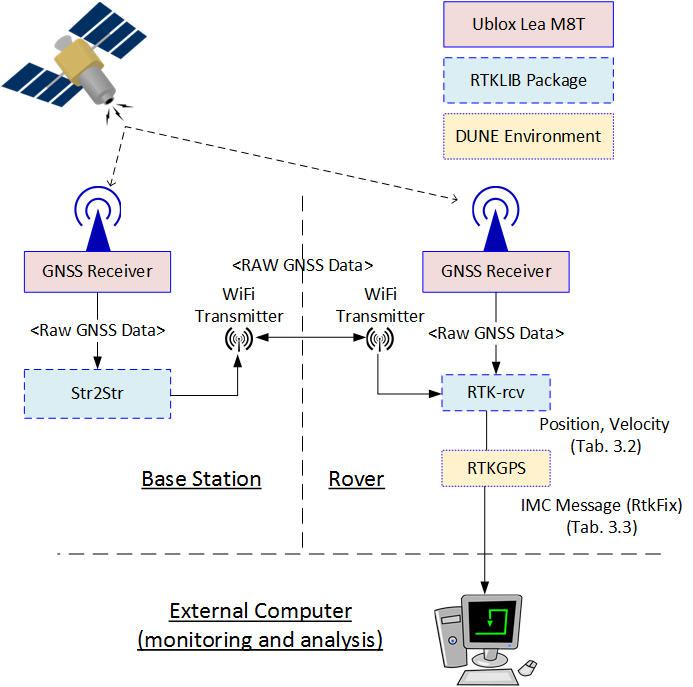
\includegraphics[width=1\textwidth]{figs/RTKLIB.png}
		\caption{The communication structure of \gls{rtklib}}
		\label{figure:RTKLIB_STRUCTURE}
\end{figure}
\subsection{Rtkrcv}
As part of the \gls{rtklib} Rtkrcv is  used to calculate the position of the rover in real time. Rtkrcv can be configured to have two output streams. It's desired in a automatic landing system to have a velocity estimate. However this is not provided in the newest version of \gls{rtklib}, and therefore a altered version of \gls{rtklib} is used in the navigation system where the velocity is part of the output data. The position output is in \gls{enu} format and the full output structure is presented in table \ref{Tb:RtklibOutput}
\begin{table}[H]
\begin{center}
    \begin{tabular}{ | l | l |}
    \hline
    \textbf{Header} & \textbf{Content} \\ \hline
     1 Time & The epoch time of the solution indicate the true receiver\\& signal reception time. Can have the following format:\\&\\& yyyy/mm/dd HH:MM:SS.SSS:\\& Calender time in GPST, UTC or JST.\\&\\&
     
     WWWW SSSSSSS.SSS:\\&
     GPS week and TOW in seconds  \\ \hline
     2 Receiver Position & The rover receive antenna position \\ \hline
     3 Quality flag (Q) & The flag which indicates the solution quality.\\& 1:Fixed\\& 2:Float\\& 5:Single \\ \hline
     4 Number of valid satellites (ns) & The number of valid satellites for solution estimation. \\ \hline
     5 Standard deviation & The estimated standard deviation of the\\& solution assuming a priori error model and error\\& parameters by the positioning options \\ \hline
     6 Age of differential & The time difference between the observation data epochs\\& of the rover receiver and base station in second. \\ \hline
     7 Ratio factor & The ratio factor of "ratio-test" for standard integer\\& ambiguity validation strategy \\ \hline
     8 Receiver velocity & The velocity of the rover. Given only when output is\\& in enu format \\ \hline
    \end{tabular}
\end{center}
\caption{Rtklib output solution format }
\label{Tb:RtklibOutput}
\end{table}
\subsection{Str2str}
Str2str is used as a base station program that can receive raw \gls{gnss} data and further export data over tcp, set-up by str2str. Str2str sends out Radio Technical Commission for Maritime Service 3 (RMTC3) formatted messages, however it can be configured to send whatever comes in as input. The communication between str2str and rtkrcv is shown i figure \ref{figure:RTKLIB_STRUCTURE}
\section{Ardupilot}

\section{JSBsim}
JSBSim \citep{berndt2004jsbsim} is an open-source flight dynamic model that is able to simulate a physical model of an arbitrary aircraft without the need of specific compiled and linked program code. The simulator is design such that a third party software e.g. Ardupilot can expose the model to external forces and moments. This enable \arcfull{sil} testing of system that is able to run in a hardware configuration with only minor configuration alteration.
\cleardoublepage
%\part{Method}

\chapter{Landing path}\label{Ch:LandingPath}
The path generator in the  autonomous landing system is designed to enable \gls{uav} landing in both a stationary and a moving net. The path is created in two main stages. The first is the creation of the virtual runway, which is defined as a straight line along the heading of the net, as shown in figure \ref{Fig:LandingPhase}. The second stage apply a lateral Dubins path \ref{S:DubinsPath} and longitudinal straight line path to create a path that ensures that the \gls{uav} is able to enter the straight line along the virtual runway at the correct height and attitude. The design is inspired by the work done in \citep{Skulstad&Syversen} were way-points was used to guide the \gls{uav} toward the landing approach.
\section{The virtual runway}\label{SS:netApproach}
The virtual runway is inspired by the work done in \citep{Skulstad&Syversen} where waypoint was used to create a straight line path towards the net. This method proved successful, and since the \gls{uav} descent towards the net should be as controlled as possible only small angles is used when transitioning between way-points. The straight line path is constructed relative to the net as shown in figure \ref{Fig:LandingPhase}, with way-points given as:
\begin{subequations}
\begin{align}
&\mathbf{WP4} = 
\begin{bmatrix}
-a0 \\
0 \\
h_{nc} + a1\tan(\gamma_a) 
\end{bmatrix}\\
&\mathbf{WP3} = 
\begin{bmatrix}
a1 \\
0 \\
h_{nc} - a1\tan(\gamma_a)
\end{bmatrix}\\
&\mathbf{WP2} = \mathbf{WP3} + 
\begin{bmatrix}
a2 \\
0 \\
a2\tan(\gamma_d)
\end{bmatrix}\\
&\mathbf{WP1} = \mathbf{WP2} + 
\begin{bmatrix}
a3 \\
0 \\
0 \\
\end{bmatrix}
\end{align}
\end{subequations}
were the description of the parameters used is given in table \ref{Tb:Approach Parameters}. The net is placed between the fourth and third way points such that transitional behaviour do not occur during the finale stage of the net landing. In addition the path has been made with the assumption that the $\gamma_a$ and $\gamma_d$ is considered small. This assumption is made to ease the demand of the controllers used in the landing system.
\begin{table}[H]
\begin{center}
    \begin{tabular}{ | l | l |}
    \hline
    \textbf{Parameter} & \textbf{Description} \\ \hline
    $a0$ & The distance behind the net \\ \hline
    $a1$ & The distance in front of the net \\ \hline
    $a2$ & The length of the glide slope \\ \hline
    $a3$ & The length of the approach towards the glide slope \\ \hline
    $\gamma_a$ & The net attack angle \\ \hline
    $\gamma_d$ & The glide slope angle \\ \hline
    \end{tabular}
\end{center}
\caption{Net approach parameters }
\label{Tb:Approach Parameters}
\end{table}
The way point vectors are rotated into the NED frame by a rotation around the z-axes.
\begin{equation}
WP^n = R(\psi_{net})WP^b
\end{equation}
were $\psi_{net}$ is the heading of the net, and $R(\psi_{net})$ is the rotation matrix around the z-axis.
\begin{figure}\label{Fig:LandingPhase}
\def\svgwidth{\textwidth} % Defining the width since Inkscape hasn't done this yet in the .pdf_tex file
\input{InkFig/LandingPhase.pdf_tex}
\caption{The virtual runway}
\end{figure}

\section{The landing path}\label{SS:LandingApproach}
The landing path is separated into two parts, which is a lateral and longitudinal path. The path is designed to ensure that the \gls{uav} follows the path along the virtual runway it must be at the correct height with the correct attitude from any initial position. In addition it's desirable that the decent angle is kept small to ease the strain on the control system, and reduce chance of overshoot of way-points.
\subsection{Lateral path}
The lateral path is designed as a Dubins path, where the initial position is the start pose and the final pose is the start of the virtual runway. Dubins path was chosen due to it's simplicity in description and it fulfils the requirement that it's smooth enough for path following.
\subsection{Longitudinal path}
The longitudinal path is designed as a straight line along the lateral path, which results in a spiral path in the arcs created by Dubins path. The path hold a constant decent angle until the correct height is reached, which is defined as the start height for the virtual runway.
\begin{equation}
r(i+1) = r(i) +
\begin{bmatrix}
0\\
0\\
||p(i)||_2\tan(\gamma_d)
\end{bmatrix}
\end{equation}
where $r(i)$ is the landing path and 
$p = \begin{bmatrix}
x(i) & y(i)
\end{bmatrix}^T
$

The lateral path was chosen for the autonomous landing system is Dubins path, due to it's simplicity in description and it fulfils the requirement that it's smooth enough for path following. Since it's desired for the \gls{uav} to decent with small decent angle the longitudinal path is constructed with straight lines. Combined with Dubins path, the circles in the start and end of the path becomes spirals. This increase the demands on the controllers used, since they has to both control the heading in addition to the decent rate with the same control surface. This is the main reason for small angles in the longitudinal path.

The path generation system is designed such that the operator can choose how the path should be generated. The system allows for manual creating of the path, or simply create the shortest path from the start pose to the end pose, which is the first way-point in the path towards the net.
%\chapter{Navigation system}
The navigation system apply \gls{rtk-gps} for position and velocity measurement, which provide higher position accuracy then a standalone \gls{gps}. However the \gls{rtk-gps} is subject to drop out, which create a situation where the navigation system should switch to standalone \gls{gps} or wait for the \gls{rtk-gps} to return. A state machine has been created to handle the state switching between \gls{rtk-gps} and the external navigation data, which is navigation data from the Pixhawk. This is handled in two steps. The first is a short loss compensator stage, where the backup standalone \gls{gps} is compensated to get a position solution closer to the \gls{rtk-gps} solution. The second stage fully disconnect the \gls{rtk-gps}.
\section{Navigation state}\label{S:NavState}
The navigation system consists of five states, which is controlled by a state machine. The state transitions are determined by what's available and what the operator has specified should be used. The output from the state machine is the IMC message EstimatedState, which is the only state source used in the Dune system. The state machine also dispatch a IMC message that informs which the source used in the navigation system, and which sources is available. Currently only the \gls{rtk-gps} system is considered as a internal system, however this can be expanded to include other sensors used in the Dune system.

The input to the navigation system is IMC message ExternalNav and GpsRtkFix. The ExternalNav message is the primary state source when the \gls{rtk-gps} is not in use, and it's receive the state information from the Pixhawk mounted in the X8.

During a short loss of the \gls{rtk-gps} the position solution in the ExternalNav message is compensated to avoid sudden change in position. The short loss compensator is explain further in \ref{ss:ShortLoss}. The short loss system is implemented to avoid drop out of the \gls{rtk-gps} when a message is delayed, or its struggling due to the dynamic behaviour of the \gls{uav}.

The state machine is depicted in figure \ref{Fig:NavState}, with the edge description given in table \ref{Tb:Nav state edge}.

\begin{figure}\label{Fig:NavState}
\def\svgwidth{\textwidth} % Defining the width since Inkscape hasn't done this yet in the .pdf_tex file
\input{InkFig/StateMachine.pdf_tex}
\end{figure}
\begin{table}[H]

    \begin{tabular}{ | p{1cm} | p{8cm} | | p{4cm} |}
    \hline
    \textbf{Edge} 	& \textbf{Event} 										& \textbf{Guard} \\ \hline
    A 				& Event: Received External Nav message 					& None \\ \hline
    B 				& Time out: Fix \gls{rtk-gps} solution for $x$ seconds 	& None \\ \hline
    C 				& Time out: $x$ seconds since last valid GpsFixRtk 		& None \\ \hline
    D 				& Flag: Using Rtk is set true& None \\ \hline
    E 				& Flag: Using Rtk is set false& None \\ \hline
    F 				& Time out: $x$ seconds since last valid GpsFixRtk 		& Short loss compensator:\\ 
      				& Event: Received GpsRtkFix with $type==None$ 			& Enabled\\ \hline
    G 				& Event: Received valid GpsFixRtk message				& None \\ \hline
    H 				& Time out: $x$ seconds since last valid GpsFixRtk 		& Short loss compensator:\\
    				& Event: Received GpsRtkFix with $type==None$			& Disabled \\ \hline
    I 				& Time out: $x$ seconds since last valid GpsFixRtk 		& None \\ \hline
    \end{tabular}

\caption{Net approach parameters }
\label{Tb:Nav state edge}
\end{table}

\subsection{Short loss of RTKGPS}\label{ss:ShortLoss}
In the event of \gls{rtk-gps} drop out a offset can be added to the position solution in order to prevent a sudden change in position. The offset is defined as the average difference between the $N$ latest position solution from the \gls{rtk-gps} and the external navigation system:
\begin{equation}
offset = \frac{1}{N}\sum_{n=0}^N(RTKGPS(n)-External(n))
\end{equation}
where the \gls{rtk-gps} solution is displaced into the External nav system. However during the implantation it was discovered that the standard displace function in the DUNE literary was inaccurate in correctly calculating the hight of a offset point. The problem was that the geodetic latitude calculation was calculate assuming that the Earth has a spheric shape. This was solved by creating a new displace function where the geodetic latitude is calculated in according to
%\chapter{System}
This chapter contain the description for the system used in the autonomous landing system.
\section{Navigation system}
The navigation system used in the autonomous landing system consist of two sensor packages. The first is part of the pixhawk (REF TIL PIXHAWK), and the other is a Ublox Lea M8T \gls{gnss} receiver suplemented with the open source program RtkLib. The system apply RtkLib for more accurate position and velocity estimation through the use of \gls{rtk-gps}. The output from the RTKGPS software contains only the relative position from the base station, and not the position of the base station. Therefore a task was created to send the global base station location to the navigation system, which enable the rest of the system to calculate the global position of the uav.

The base station position is received in the RTKGPS task in DUNE, were it's included in the GpsFixRtk message.

A task in the nest receive the gps position of the base, and the operator can monitor it in neptus. When the operator choose to fix the base station gps position a parameter update is send to the task, which will start to send a gpsfixrtk message to the uav. 

TODO: Create figure that shows the information flow that is used to create the rtkfix message.
\subsection{Navigation source}
The navigation system is able to receive data from two separate sensor system, which is the Pixhawk package and the Ublock \gls{gnss} receiver with RTKLib. The output from RTKLib is only available if the \gls{rtk-gps} solution is fixed. The default configuration is that the position solution is received from the Pixhawk.

\subsection{Base station}
The base station is able to send it's own gps position to the \gls{uav}. The operator can decide when the base station could be considered as fixed.
\subsection{Operator interface}
The operator use the Neptus platform as operational interface during the landing. The console includes information about the position of the uav, as well as the source of the position measurement. The operator can monitor the status of the gps system, including what is accepted by the navigation system. During a autonomous landing the operator must be fully aware of the status of the navigation system, such that an abort due to lost gps fix. This system can be expanded to include other sensors, like a ranging system, IMU, camera ex.
%\subsection{Position correction}%Flytt til resultat
%The highly dynaimcal nature of the uav create a challenge for the navigation system due to the blocking of the gps antenna from the satellite constellation. The problem was reduced by using a gps receiver that has a high performance in satellite tracking, however this does not remove the problem. A float solution from the gps system is valid for some seconds after fix is lost, due to the predictive nature of the Extended Kalman filter in rtklib. However after a seartin amount of time the navigation system swithces over to use the position estimate from the pixhawk, which has a lower accuracy level then the rtk gps system. To increase the accuracy level a offset solution is proposed. By calculating the difference between the fixed rtk gps solution and the position solution from the pixhawk a offset can be found. If the offset can be assumed constant or quasi stationary it can be used to increase to accuracy level for the navigation system enough to allow for completion of critical phases of a manoeuvre. However tests showed that the offset was not constant nor quasi stationary. By applying the offset to the pixhawk position solution the accuracy level will increase, but not enough to allow for execution of critical manoeuvres.
%In order to make the navigation system more robust, some methods was explored. 
\section{Path generation}
The landing plan is design with the assumption that the aerial space in which the uav operates is limited. The limitation can be the range of the uav, regulatory limits or weather. In addition the autonomous landing system must be able to perform a safe landing from any initial position. Furthermore the size of the virtual run way should be constructed by the operator. The type of uav operation dictates the maximum size of the landing path. Different types of uav operation is LOS, ELOS, BLOS and BRLOS. Only the first is considered in this thesis, which means that the pilot must have the uav in view during the entire flight. The operator must also be able to control the angle which the uav is descending, which means that the height of the landing path is fixed. Therefore the uav must be at the correct altitude before it can start descending toward the landing net.

A landing plan that is proposed consist of Dubins path \ref{S:DubinsPath} in the lateral plane, and straight lines in the longitudinal plane. The path is generated from an arbitrary start positing, and will create a continuous path toward the landing approach. The design is inspired by the work done in \citep{Skulstad&Syversen} were way-points was used to guide the uav toward the landing approach.

The plan is generated in a Dune task which receive a plan generation request from Neptus. Then a plan is created, which is sent to the Dune task Plan manager, which in turn sent desired state to the guidance system. The plan is decoupled from the guidance system, which allow for use of different control design when executing the landing plan.

The Dubin path is constructed with a followPath manoeuvre.

The landing plan generated by the Dune task can be requested for review by the operator in Neptus. The plan will not start before the operator has reviewed the plan, and approved by uploading it to the uav. In the uploaded version a specification list on which controller that should be used is included.  
\subsection{The net approach}
The net approach path consist a straight line in the lateral plain, and straight lines in the longitudinal plane. The net approach way-points are defined relative to the position of the net, which has been defined as origo. The four way-points in the net approach is defined as follows:
\begin{subequations}
\begin{align}
&\mathbf{WP1} = 
\begin{bmatrix}
-a0 \\
0 \\
h_{nc} + a1\tan(\gamma_a) 
\end{bmatrix}\\
&\mathbf{WP2} = 
\begin{bmatrix}
a1 \\
0 \\
h_{nc} - a1\tan(\gamma_a)
\end{bmatrix}\\
&\mathbf{WP3} = \mathbf{WP2} + 
\begin{bmatrix}
a2 \\
0 \\
a2\tan(\gamma_d)
\end{bmatrix}\\
&\mathbf{WP4} = \mathbf{WP3} + 
\begin{bmatrix}
a3 \\
0 \\
0 \\
\end{bmatrix}
\end{align}
\end{subequations}
were the description of the parameters used is given in table \ref{Tb:Approach Parameters}. The net is placed between the first and second way points such that transitional behaviour do not occur during the finale stage of the net landing. In addition the path has been made with the assumption that the $\gamma_a$ and $\gamma_d$ is considered small. This assumption is made to easy the demand of the controllers used in the landing system.
\begin{table}[H]
\begin{center}
    \begin{tabular}{ | l | l |}
    \hline
    \textbf{Parameter} & \textbf{Description} \\ \hline
    $a0$ & The distance behind the net \\ \hline
    $a1$ & The distance in front of the net \\ \hline
    $a2$ & The length of the glide slope \\ \hline
    $a3$ & The length of the approach towards the glide slope \\ \hline
    $\gamma_a$ & The net attack angle \\ \hline
    $\gamma_d$ & The glide slope angle \\ \hline
    \end{tabular}
\end{center}
\caption{Net approach parameters }
\label{Tb:Approach Parameters}
\end{table}
The way point vectors are rotated into the NED frame by a rotation around the z-axes.
\begin{equation}
WP^n = R(\psi_{net})WP^b
\end{equation}
were $\psi_{net}$ is the heading of the net.
\begin{figure}
\def\svgwidth{\textwidth} % Defining the width since Inkscape hasn't done this yet in the .pdf_tex file
\input{InkFig/LandingPhase.pdf_tex}
\end{figure}

\subsection{The landing path approach}
In order for the \gls{uav} to be able to start the landing approach the \gls{uav} must be at the correct altitude with the correct orientation from any initial position. That require a path which the \gls{uav} is able to follow. The problem can be separated into two parts. The first is the longitudinal parts, while the other is the lateral. The longitudinal path will be more exposed to large changes in heading, which puts demands of the type of path that can be chosen. However since a time demand is not required the problem becomes a path following problem. The problem has been solved by creating a Dubins path in the longitudinal plane.

A desired behaviour in the lateral plane is that the \gls{uav} should have a controlled decent. Given this desired behaviour it was decided that the lateral plane should be a glide slope, which means that the decent angle can be considered small. The strategy chosen to solve this problem is the use of straight lines in the lateral plane. The straight lines are is included with Dubins path such that the turn in Dubins path becomes a spiral.

At the end of Dubins path the path is checked if the correct height has been reach. If the correct height has not been reached the path will create a spiral that converge to the correct height. When the correct height has been reach a last arc is created in order for the \gls{uav} to get the correct orientation.

The landing path can be created in two modes, which is manual or automatic. The manual mode allow the operator to design the landing path by defined the turning direction for the start and final circle. This enable the operator to specify a path that fills a operational demand, which would not necessary be the path when in automatic.

In automatic mode all four variants, which is given in table \ref{Tb:DubinsTurningDirection}, calculated. After the length of the paths are calculated, where the shortest path is chosen to be the landing path.
The landing path approach can be generated in to different way. One mode allow for manual deciding which side the start and finish circle should be in respect on the start pose, and the net landing approach. This allow the operator full control over the landing path, and can choose a landing path that is operation feasible and not necessary the shortest path. 
\subsubsection{Extra way point}
To ensure that the path generation system will generate å flyable path an extra way point is added in the case of the start pose in cause an infeasable dubins path, or an spesial case of Dubins path which has not been implemented. The two case are
\begin{subequations}
\end{subequations}
\section{Evasion}
To ensure the safety of the operator a evasion controller is used to abort the landing when a successful landing is deemed infeasible or improbable.

\section{Guidance system}
The guidance system consist of two part. Sliding mode controller, and a los controller

\subsection{Sliding mode controller}
For course control the system use a sliding mode controller that was proposed in the paper \citep{fortuna2015cascaded}, which USGES stability property.
\begin{subequations}
\begin{align}
\dot{x} &= V_a\cos(\psi) + W_x = V_g\cos(\psi) \\
\dot{y} &= V_a\sin(\psi) + W_y = V_g\sin(\psi) \\
\dot{phi} &= \frac{g}{V_a}\tan(\varphi) \\
\dot{\varphi} &= -\frac{\varphi-\varphi_{cmd}}{T_\varphi} \\
W &= \sqrt{W_x^2 + W_y^2}
\end{align}
\end{subequations}
\begin{equation}
\epsilon(\varphi) = \begin{cases}
\cos(\varphi), & \text{if}\ |\cos(\varphi)|\geq\epsilon'\\
\epsilon', & \text{if}\ 0 \leq \cos(\varphi) < \epsilon' \\
-\epsilon', & \text{if} -\epsilon'<\cos(\varphi) < 0
\end{cases}
\end{equation}
\begin{equation}
\chi = \tan^{-1}(\frac{\dot{y}}{\dot{x}})
\end{equation}
\begin{equation}
\dot{\chi} = \frac{g\sin(\varphi)(V_a + \cos(\psi)W_x + \sin(\psi)W_y}{\epsilon(\varphi)V_g^2}
\end{equation}
\begin{subequations}
\begin{align}
\chi_d &= \tan^{-1}(-\frac{t}{\Delta} \\
\dot{\chi_d} &= -\frac{\Delta}{\Delta^2+y^2}\dot{y} \\
\ddot{\chi} &= \frac{\Delta}{(\Delta^2 + y^2)^2}(2y\dot{y}^2 - (\Delta^2 + y^2)\ddot{y})
\end{align}
\end{subequations}
\begin{equation}
\tilde{\chi} = \chi - \chi_d
\end{equation}
\begin{equation}
s = \dot{\tilde{\chi}} + \lambda\tilde{\chi}
\end{equation}
\begin{equation}
u = -\lambda\dot{\tilde{\chi}} - \rho\text{sgn}(s) - K_ds
\end{equation}
\chapter{Implementation}
This chapter contain the technical specification of the navigation system and landing path system, in addition to the payload installed in the X8 and both nests.
\begin{figure}[H]
	\centering
		\includegraphics[width=1\textwidth]{figs/DUNESystem.png}
		\caption{A simplified figure of the Dune auto land system}
		\label{figure:RTKLIB_STRUCTURE}
\end{figure}
\section{Landing path}
The landing path is specified through the Neptus plug-in LandmapLayer, which allow for real time setting of the parameters used to create the landing path. In addition the plug-in display the position of the net in the graphical map interface which is a part of Neptus. The plug-in dispatch the \gls{imc} message, LandingPlanGeneration, which has been created specifically for landing path purpose.

The \gls{imc} LandingPlanGeneration message is dispatch to the Dune system, where it's picked up by the Dune task LandingPlan. This trigger the generation of the landing path, and depending on the configuration of the Dune task and desired setting in the LandingPlanGeneration message different landing path is generated. The different variants is categorised into two groups; configuration of the Dubins path, and configuration of the virtual runway. The configuration option that result in different variants of the landing path is given in table \ref{Tb:DubinConfig}. In addition the Dune task can be configured for a dynamical landing. When configured as dynamical it's assumed that an other task is responsible for the final landing part. Therefore the vertical runway is not part of the plan, however the first part of the path is still included.
\begin{table}
\centering
\begin{tabular}{| p{2.7cm} | | p{6cm} |}
\hline
\textbf{Parameter name} 							& \textbf{Action} \\ \hline
 Automatic (boolean)								& If true a standard path where the shortest Dubins path is chosen. Otherwise a user specific path is chosen \\ \hline
Start circle turning counter clockwise (boolean)	& If true the start arc is created such that the turning direction is counter clockwise. Otherwise clockwise. Require Automatic==false \\ \hline
Finish circle turning counter clockwise (boolean)	& If true the finish arc is created such that the turning direction is counter clockwise. Otherwise clockwise. Require Automatic==false \\ \hline
Wait at loiter (boolean)							& If true a unlimited loiter is included in the path before the path continue with the path along the virtual runway. \\ \hline

\end{tabular}
\label{Tb:DubinConfig}
\end{table}

A design choice allows for user determined rotation direction. By setting the "automatic" flag to false in the \gls{imc} message LandingPlanGeneration the rotation direction is determined by the flags "startCounterClockwise" and "finishCounterClockwise".


When generated the plan must be started from Neptus, where the desired control configuration is added to the path.

A loiter manoeuvre can be included in the landing plan before the start of the path along the virtual runway. The loiter manoeuvre can be used to control when the \gls{uav} should start it's final approach, which is practical when performing a dynamical landing.
\section{Navigation system}
The navigation system is control by a state machine \ref{S:NavState}, which is used to control the content of the output \gls{imc} messages EstimatedState and NavSources. Depending on which state the navigation system is in the \gls{imc} EstimatedState message will either have position solution form the \gls{rtk-gps} system or the external navigation system. During a short loss of the RTK the external navigation position is compensated with the average difference between the RTK solution and the external navigation solution.
\subsection{RTK-GPS system}
The \gls{rtk-gps} solution is dispatched from the DUNE task RTKGPS, however before the message is accepted by the Navigation task the message must include a valid base station position. The base station position is not included in the output message from RTKlib, which demand the base station position to be calculated locally at the base station as a standalone \gls{gnss} receiver. For this purpose the DUNE task BasestationFix is used to lock the current position of the base station, which result in the base station position being transmitted to the RTKGPS task.
The navigation system require to now the reference position of the base station in order to use the \gls{rtk-gps} solution. However the base station position is currently not part of the output message from rtkrcv. This is resolved by allowing the base station to calculate it's own position as a standalone \gls{gps}. The \gls{gps} position is transmitted to a local Dune task on the base station, where the operator can decide when the base station can be considered as fixed. When the base station is considered fixed the position is sent to the X8, where it's included in the \gls{rtk-gps} solution message.
\subsubsection{Nest system}
A nest system is a stationary unit with the sole purpose of providing it's position to the rest of the Dune System. As part of the navigation system the base station is defined as a nest, where the \gls{gps} position is sent to the \gls{rtk-gps} system when fixed.
An other nest has been created to obtain the \gls{gps} position of the stationary net. The net nest is configured as a rover in \gls{rtk-gps} configuration, such that the position relative to the base station is in the same frame as the X8.
\subsection{Operator interface}
The state of the navigation system is monitored though a interface in Neptus. The interface indicate which source the Dune system is using for state information. The interfaced apply a color code to indicate which source is currently in use in addition to all sensor system that are available, as seen in table \ref{Tb:Color Code}.
\begin{table}[H]
\begin{center}
    \begin{tabular}{ | l | l |}
    \hline
    \textbf{Color} & \textbf{Description} \\ \hline
    White & Not available \\ \hline
    Yellow & Available, but not in use \\ \hline
    Green & Available, and in use \\ \hline
    \end{tabular}
\end{center}
\caption{Net approach parameters }
\label{Tb:Color Code}
\end{table}
%\chapter{SIL test}
The system was tested through a Software In the Loop (SIL) simulation. In a SIL simulation the same code that runs in the hardware is tested against a simulator which behave similarly to the real system.

\section{Path planing SIL}
The landing path is tested in both guided and FBWA. 
\section{Navigation SIL}
The navigation system was tested by creating a \gls{rtk-gps} simulator. This allowed for testing of the navigation interface, including the fixing of the base station position.

\subsection{Short rtk loss compensator}
The short rtk loss compensator was tested by adding a bias in the position solution from the simulated GpsFixRtk message. 
\chapter{Experiment}
\section{Path}
\subsection{Landing path with pixhawk autopilot}
A landing path was create with the goal of testing the concept of the landing path system. The test was perform with the pixhawk autopilot, and navigation system. Thus high performance from the X8 is not expected. The path was create in cooperation with the operator and pilot, which dictated the maximum size of the landing path.

The height where the \gls{uav} held after the approach path was to low, and during a real landing would cause the \gls{uav} to crash. Thus either the length of the landing path or the glide slope angle has to increase. The performance of the pixhawk autopilot was not adequate to successfully hit the net.

The wind condition was measured to be $5m/s$ from the north, which caused the \gls{uav} to have to perform the landing with a cross wind.

The path was created with manually deciding the rotation directions, due to the start position and where the operator wanted the \gls{uav} to circle down to the correct height. In this case the shortest path would bring the \gls{uav} close to a no-fly zone


\begin{figure}[H]
	\centering
		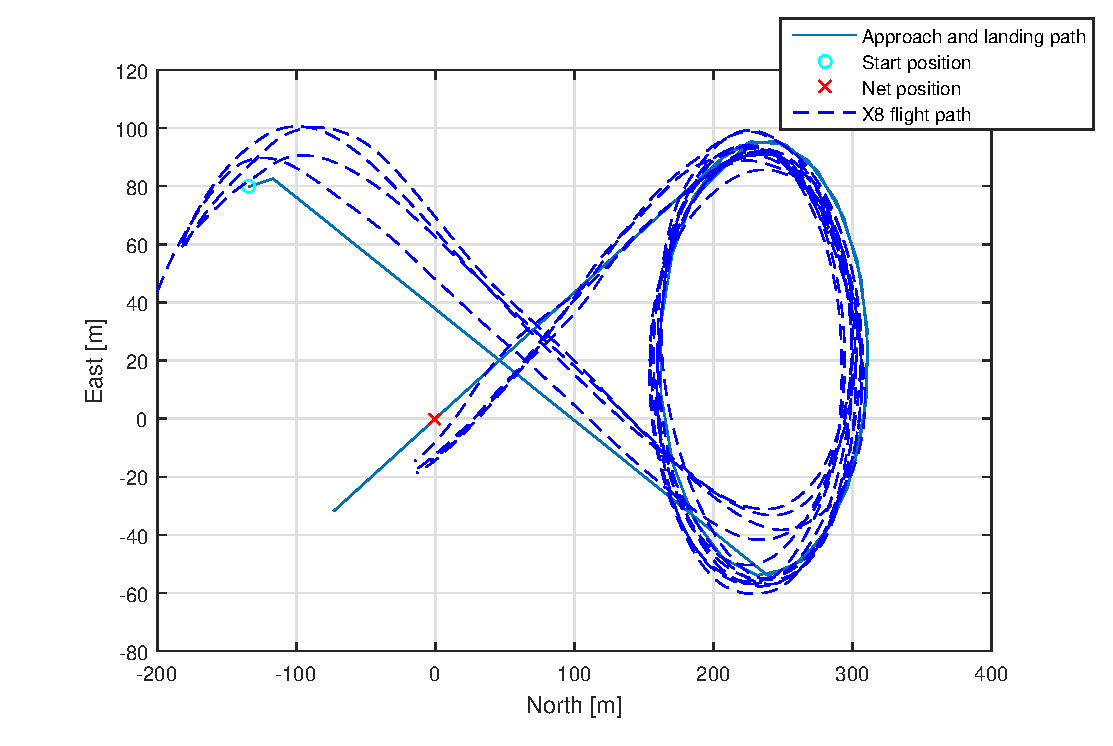
\includegraphics[width=1\textwidth]{figs/Experiment/NorthEastLandingPathArdu.eps}
		\caption{Four lateral flight paths towards the net position}
		\label{Fig:NorthEastArdu}
\end{figure}
\section{Navigation}
The navigation system was tested in both a X8 and in a multicopter system.

\subsection{Formation position}
The accuracy of the \gls{rtk-gps} position system was tested with two mutlicopter system, with the goal of measuring the distance between them. During stationary conditions it was determined that \gls{rtk-gps} was highly accurate, and is required when performing a formation flight. The same principle is used in determining the net position, where the net nest apply \gls{rtk-gps} to determine it's own position. However currently the position has to manually be written to Neptus, which must change when performing a ship landing.
\subsection{Short loss compensator}
Include result when short loss was not in use. Compare to result when it's in use.

The short loss compensator bring the position solution from the pixhawk close enough to the \gls{rtk-gps} solution such that the navigation system does not lose its position. However a highly aggressive control system that attempt to keep the error at centimeter level is expected to react to the discontinues introduced from the compensator. All though currently it has not been concluded that the compensator cause problems for the control system, since failure has happen during demanding wind condition. 
\chapter{Conclusion and recommendation for further work}
\section{Conclusion}
This thesis has implemented and tested a path and navigation system for autonomous landing of fixed-wing \gls{uav} in a stationary net. The design of the landing plan generation allowed for the generation of landing waypoints, used to create a flyable path for the \gls{uav} from an arbitrary position and direction. The parametrisation of the landing waypoint is accessed through the landing plan generator \gls{api}, which allows for specification of key factors in the creation of the landing plan, e.g. the length of the landing path, decent angle and rotation direction in the approach path.

The navigation system has successfully been integrated with \gls{rtk-gnss}, which has been added as a state in the new navigation state control system implemented in this thesis. The effect of short loss of \gls{rtk-gnss} lock has been mitigated with the implementation of a robust \gls{rtk-gnss} system, which fuse navigation data from an secondary \gls{gnss} system together with the \gls{rtk-gnss} navigation data into a compensator for the external navigation system in the \gls{uav}. The compensator showed that it was able to prevent loss of position accuracy in a short duration after \gls{rtk-gnss} drop out.

Field experiments at Agdenes of the autonomous landing system was performed with a virtual net placed above the runway. The performance of the control system showed promising results, however the low level controllers must be fined tuned for autonomous flight operation. The navigation system with \gls{rtk-gnss} tested in the field at Agdenes showed excellent result during testing of the autonomous stationary net landing system.

The mobile sensor unit showed excellent performance when used as position reference for the stationary net placement. The functionality of the mobile sensor unit can be expanded to be closer integrated into the autonomous landing system.

%From the experimental testing of the autonomous landing system it's concluded that both the lateral and longitudinal control system can be used in the autonomous landing system, however further tuning of the low level controller are required. In addition to further testing of the autonomous landing system in order to determine


%The navigation system with \gls{rtk-gnss} tested in the field at Agdenes showed excellent result during testing of the autonomous stationary net landing system.



%The implementation of the landing plan generator presented in Ch. \ref{Ch:Implementation} showed that the landing path generator can be configure through the use of the \gls{api} in the form of the \gls{imc} message LandingPlanGeneration, which ensures that the parameters used to create a landing plan is available in the fixed structure of the \gls{imc} protocol. Further the Software In the Loop (SIL) simulation of the autonomous landing system presented in section \ref{ss:SILLandingPlan} showed the the presented system is capable of performing a autonomous landing in a stationary net with a landing plan created from a arbitrary location. The testing of the control system used in the autonomous landing system showed that during a simulation the control system is able to pass through the net with acceptable precision.
%
%
%In Ch. \ref{Ch:Implementation} the necessary navigation systems need to perform a autonomous landing operation was presented. The \gls{rtk-gnss} system is able to provide high accurate position solution of the \gls{uav} relative to the base station position, with the mobile sensor unit providing a reference position for net placement. The navigation source monitor in Neptus provide the operator with feedback on the state of the \gls{uav} navigation system, which enable the operator to make informative decisions during a autonomous landing in a stationary net operation.
%
%
%The results from the experimental testing of the autonomous landing system presented in Ch. \ref{Ch:ExperimentalTesting}, shows that the lateral control system is capable of performing a autonomous landing during strong wind condition, given that the lateral control system is tuned for the current wind condition. A proposed strategy for tuning the lookahead distance of the lateral control system include a lookahead distance which is a function of the cross track error of the desired path. The longitudinal control system had a stable performance during the experimental testing, which resulted in a low variance in the average height errors. However the high average height error results from the autonomous landing missions showed that longitudinal control system was slow to converge to the desired height. A tuning attempt performed in the the SIL simulation in section \ref{ss:SILLandingPlan}, where the time constant for the height reference smoothing filter was reduced, showed promising results. However due to time limitation the new time constant has not been tested in the field, and together with further tuning of the low level pitch controller in the \gls{uav} would result in a performance closer to that in the SIL simulation.
%
%
%The performance of the navigation system presented in Ch. \ref{Ch:ExperimentalTesting} shows that the navigation system with \gls{rtk-gnss} is reliable enough to be used during a autonomous landing operation. The \gls{rtk-gnss} is still prone to drop out due to shift in satellite geometry, however with the introduction of the short \gls{rtk-gnss} compensator a short loss of \gls{rtk-gnss} is handled in a way that keeps \gls{rtk-gnss} availability and position accuracy. The short \gls{rtk-gnss} loss compensator was introduced in section \ref{ss:ShortLoss} as a method of exploiting the slow moving difference between the \gls{rtk-gnss} and the external navigation system by fusing navigation data from the \gls{rtk-gnss} and the secondary \gls{gnss} system together in a compensating term for the external navigation system.
%
%
%The introduction of the mobile sensor unit in section \ref{ss:MobileSensor} has provide a reference position for net placement in Neptus, in order for correct placement of the landing path. The introduction of a mobile sensor that act as a reference position for net placement allows for increase operational control over a autonomous landing operation, thus reducing the risk of a undesired landing plan being created due to wrong placement of the net.
%During the experimental field test in Ch. \ref{Ch:ExperimentalTesting} at Agdenes airfield limitation in the start height of the landing path when attempting a landing from East was discovered. Due to a surrounding environment which demand a high start altitude, a landing plan created with the purpose of landing in a real stationary net would strain the operational restriction of flying a Line Of Sight operation. In the event a autonomous landing from East is attempted with the current control system the entire runway at Agdenes must be used to ensure a long enough glide slope for sufficient altitude decrease. Alternative landing direction from the west has the disadvantage of being the typical direction of the wind, which is undesired when attempting a autonomous landing due to increased ground speed. All thought during calm wind periods this would not prove a problem, thus becoming an attractive alternative due to the allowance of a lower start altitude of the landing path.
%
%Due to limited time for experimental testing the full potential of the autonomous landing system has yet to be determined, together with a landing attempt in a real stationary net. The overall performance of the autonomous landing system has shown that the system is capable of performing a autonomous landing in a stationary net.


\section{Recommendation for further work}
This master thesis has presented a autonomous landing system, with the main focus on the path and navigation system.
The most important focus for further work is the tuning of the low level controllers in the X8 for autonomous flights. An important aspect here is the separation between control parameter for autonomous and manual flight. Thus the control system must be able to switch tuning parameters depending on the mode of Ardupilot. Further work on the lateral controller would be a lookahead distance parameter which is a function of the cross track error relative to the desired lateral path. In addition the lateral control system could be improved to better follow a path through a turning manoeuvre, with the main motivation of reducing overshot.

In order to shorten the distance of the landing path, a new type of longitudinal control system can be investigated with the main motivation being to use the high dynamic behaviour of the X8 to more effective decrease the altitude. The new control design would use a higher attack angle, however due to the increase stress on the wings the controller must be time dependent to prevent a crash.

The \gls{uav} navigation system can be improved by expanding the functionality of the short \gls{rtk-gnss} loss compensator, with the goal of creating a more robust \gls{rtk-gnss} system. The improvement could be the use of the velocity information from the external navigation system together with the compensator term to further increase the duration where the short \gls{rtk-gnss} loss compensator is valid.

The functionality of the mobile sensor unit can be expanded to enable the fixed wing \gls{uav} to apply target tracking of the position of the sensor unit. This could be used in a autonomous net landing system where the position of the net is dynamic, without the use of multirotor \glspl{uav}. This can be used in a autonomous landing system where the net is placed on a ship.

The autonomous landing system in a stationary net require a monitor to follow the fixed wing \gls{uav} along the landing path and detect when the \gls{uav} hit the net, or be used to trigger an abortion. In the case of abortion the autonomous landing system must include a evasive manoeuvre, however further testing of the current landing system is required to find the boundaries of when an abortion should be triggered.
%\include{Discusion}
%% include here the other chapters

\renewcommand*{\bibname}{References}
\bibliographystyle{plainnat}
\bibliography{main}

%% Uncomment the following if you have any appendix
 \appendix
 \addtocontents{toc}{%
  \protect\vspace{1em}% 
  \protect\noindent \bfseries \appendixtocname\protect\par
  \protect\vspace{-.5em}%
 }
 \renewcommand{\chaptername}{\appendixname}
%% include below possible appendices (chapters)
\chapter{Landing plan generation API}\label{AP:APIIMC}
The landing plan generator \gls{api} consist of the \gls{imc} LandingPlanGeneration, given in table  the field with description is given in table \ref{ApTb:LandingPlanAPI}.
\begin{table}
\centering
\begin{tabular}{| p{4cm} | p{2cm} | p{6cm} |}
\hline
\textbf{Field name}	& \textbf{Type}	& \textbf{Description} \\ \hline
Command								& Enumerated	& Command the plan database to generate the plan, with the option of executing the plan after generation. \\ \hline
Operation							& Enumerated	& Type of operation started.	\\ \hline
Plan identifier						& Plain text	& Plan identifier.	\\ \hline
Reference latitude					& rad			& Reference latitude for the landing path.	\\ \hline
Reference longitude					& rad			& Reference longitude for the landing path.	\\ \hline
Reference height					& m				& Reference height for the landing path.	\\ \hline
Height over ground					& m				& Offset from the reference height to placement.	\\ \hline
Reference point heading				& rad			& Heading of the reference point in NED frame.	\\ \hline
Distance behind						& m				& Aiming point behind the reference point.	\\ \hline
Final approach length				& m				& The length of the final approach towards the reference point.	\\ \hline
Final approach angle				& rad			& The decent angle of the final approach vector. 	\\ \hline
Glide slope length					& m				& The length of the glide slope in the landing path.	\\ \hline
Glide slope angel					& rad			& The decent angle of the glide slope.	\\ \hline
Approach decent angle				& rad			& The decent angle of the approach path.	\\ \hline
Approach length						& $m$			& The length of the vector from the end of the approach path to the glide slope.	\\ \hline
Landing speed						& $m/s$			& The landing speed.	\\ \hline
Approach speed						& $m/s$			& The approach speed.	\\ \hline
Start turning circle radius			& m				& The radius of the first turning circle.	\\ \hline
Finish turning circle radius		& m				& The radius of the second turning circle.	\\ \hline
Automatic generate landing plan		& Flag			& The approach path will calculate the shortest path form the initial position towards the start of the landing path.	\\ \hline
Start circle turning direction		& Flag			& Manually setting the rotation direction of the first circle.	\\ \hline
Finish circle turning direction		& Flag			& Manually setting the rotation direction of the finish circle.	\\ \hline
Wait at loiter						& Flag			& Setting if after the approach path the \gls{uav} should enter a loiter manoeuvre.	\\ \hline
\end{tabular}
\caption{The landing plan generator \gls{api}}
\label{ApTb:LandingPlanAPI}
\end{table}
\chapter{Guidance and control system}
The autonomous landing system is design to be independent from any types of guidance and control system. However this hold only true when the guidance and control system is implemented in the DUNE environment due to the requirement of an accurate navigation system. The control system is separated into two groups, high level and low level control. The low level control is the control loops for the actuators, which are only controlled by ardupilot. The high level controllers depend on the the configuration of Ardupilot, which is listed in table \ref{tb:ArduPilotMode}.
\begin{table}
\centering
\begin{tabular}{| p{3cm} | p{5cm}|}
\hline
\textbf{Mode}	&	\textbf{Description} \\ \hline
Guide			& Ardupilot set-point guidance and control system 												\\ \hline
FBWB			& DUNE lateral controller with desired height controlled in a set-point controller in Ardupilot \\ \hline
FBWA			& DUNE lateral and longitudianl controller, where control input is sent directly to the low level controllers in Ardupilot 																						\\ \hline
\end{tabular}
\caption{Guidance and control modes in autopilot viable for the landing system}
\label{tb:ArduPilotMode}
\end{table}

\section{Lateral controller}
The lateral controller used in the autonomous landing system is based on the paper \citep{fortuna2015cascaded}, which is a s
\section{Longitudinal controller}
The longitudinal controller is based on the paper \citep{you2012guidance}
\chapter{Navigation performance results}\label{AP:RTKPerformance}

\begin{table}
\centering
\begin{tabular}{| l | l | l | l |}
\hline
\textbf{Nr.}	& \textbf{FIX \%}	& \textbf{FLOAT \%}	& \textbf{NONE \%}	\\ \hline
$1$				& $99.2 $	& $0.8$	& $0.0$									\\ \hline
$2$				& $100 $	& $0.0$	& $0.0$									\\ \hline
$3$				& $99.9 $	& $0.1$	& $0.0$									\\ \hline
$4$				& $99.9$		& $0.1$	& $0.0$									\\ \hline
$5$				& $100$		& $0.0$	& $0.0$									\\ \hline
$6$				& $100$		& $0.0$	& $0.0$									\\ \hline
$7$				& $99.6$	& $0.4$	& $0.0$									\\ \hline
$8$				& $99.9 $ 	& $0.31$	& $0.0$									\\ \hline
\end{tabular}
\caption{Performance of the RKT-GNSS system the first day during the executing of the landing plans}
\label{TB:RTKFirstDayLanding}
\end{table}
%\section{Landing plan parameters}

\subsection{Parameter used in experiment with ardupilot}

\begin{table}
\centering
\begin{tabular}{| p{4} | p{4} |}
\hline
\textbf{Parameter}			& \textbf{Value}			\\ \hline
Net latitude				& $64,62848193735199 \deg$ 	\\ \hline
Net longitude				& $9,726324254172361 \deg$ 	\\ \hline
Net height					& $150 m$					\\ \hline
Net height offset			& $-3 m$ (NED frame)		\\ \hline
Net heading					& $66.5 \deg$				\\ \hline
Distance behind net			& $80 m$					\\ \hline
Final approach length		& $15 m$					\\ \hline
Final approach angle		& $3 \deg$					\\ \hline
Glide slope length			& $200 m $					\\ \hline
Glide slope angle			& $3 \deg$					\\ \hline
Glide slope approach		& $10 m$					\\ \hline
Landing speed				& $16 m/s$					\\ \hline
Approach speed				& $18 m/s$					\\ \hline
Turn radius first circle	& $75 m$					\\ \hline
Turn radius final circle	& $75 m$					\\ \hline
Start turning direction		& Clockwise					\\ \hline
Finish turning direction	& Counter-Clockwise			\\ \hline
\end{tabular}
\end{table}
\chapter{Rtklib Configuration}\label{APPENDIX:RTKLIB}
This appendix chapter contain the configuration file used to configure RTKlib in the X8, which is given as:
\verbatiminput{rtkrcv.conf}

\end{document} 
